
\documentclass[french]{beamer}

\usetheme{metropolis}
\usepackage{appendixnumberbeamer}
%\usepackage[scale=2]{ccicons}
%\usepackage{minted}
%\usepackage{booktabs}
%\usepackage[scale=2]{ccicons}
\usepackage{pbox}
\usepackage{pgfplots}
\usepgfplotslibrary{dateplot}

\usepackage{xspace}
\newcommand{\themename}{\textbf{\textsc{metropolis}}\xspace}
\usepackage{pdfpages}
\usepackage{tikz}
\usetikzlibrary{backgrounds}
\usepackage{tabularx}
% Package used for highlighting
\usepackage{soul}
% Package used for multirow tables
\usepackage{multirow}
\usepackage{graphicx}
\usepackage{textpos}
\usepackage{booktabs}
\usepackage{lipsum}% http://ctan.org/pkg/lipsum
\usepackage[normalem]{ulem}
\usepackage{transparent}

%INCOMPATIBLE AVEC FOOTNOTE
%\usepackage{setspace}% http://ctan.org/pkg/setspace
\usepackage{xcolor,colortbl}
\definecolor{nla}{HTML}{E6B71F}
\definecolor{sla}{HTML}{3EA4B9}
\newcommand{\nla}{\cellcolor{nla}}  %{0.9}
\newcommand{\sla}{\cellcolor{sla}}  %{0.9}
%\usepackage[scale=2]{ccicons}
%COLORS
\definecolor{olive}{rgb}{0.3, 0.4, .1}
%\definecolor{white}{HTML}{FFFFF}
\definecolor{fore}{RGB}{249,242,215}
\definecolor{back}{RGB}{51,51,51}
\definecolor{title}{RGB}{255,0,90}
\definecolor{dgreen}{rgb}{0.,0.6,0.}
\definecolor{gold}{rgb}{1.,0.84,0.}
\definecolor{JungleGreen}{cmyk}{0.99,0,0.52,0}
\definecolor{BlueGreen}{cmyk}{0.85,0,0.33,0}
\definecolor{RawSienna}{cmyk}{0,0.72,1,0.45}
\definecolor{Magenta}{cmyk}{0,1,0,0}
\definecolor{mygreen}{HTML}{033E37}
\definecolor{myred}{HTML}{E50707}
\definecolor{mylightgreen}{HTML}{00A339}
\definecolor{greensolution}{HTML}{2AAE00}
%\usefonttheme{structuresmallcapsserif} 

%\usefonttheme{smallcapsserif} 
\usefonttheme{serif} 
%\setsansfont[BoldFont={Source Sans Pro Semibold},           Numbers={OldStyle}]{Source Sans Pro}

%\metroset{titleformat=allsmallcaps}
%\usefonttheme{serif} % default family is serif
\setbeamercolor{frametitle}{bg=mygreen}
\setbeamercolor{example text}{fg=mylightgreen}
\setbeamercolor{alerted text}{fg=myred}
\usepgfplotslibrary{dateplot}
%Prevents arrow on x axis
\pgfplotsset{ every non boxed x axis/.append style={x axis line style=-}, every non boxed y axis/.append style={y axis line style=-}}
\newcommand{\tool}[1]{\texttt{#1}\xspace}
\newcommand{\cat}[1]{\textsc{#1}\xspace}
\newcommand{\variante}[1]{\textsc{#1}\xspace}
\renewcommand*{\thefootnote}{\alph{footnote}}

% visible only on some slides tikz pictures
\tikzset{
  invisible/.style={opacity=0},
  visible on/.style={alt=#1{}{invisible}},
  alt/.code args={<#1>#2#3}{%
    \alt<#1>{\pgfkeysalso{#2}}{\pgfkeysalso{#3}} % \pgfkeysalso doesn't change the path
  },
}

% Prevent section slide 
%\newcommand{\metropolis@disablesectionpage}{\AtBeginSection
%}
\AtBeginSection[]
                  {
                    \begin{frame}{Plan}
                      \tableofcontents    [
                        currentsection
                      ]
                    \end{frame}
                  }%

\AtBeginSubsection[]
                  {
                    \begin{frame}{Plan}
                      \setbeamertemplate{section in toc}[sections numbered]
                      \tableofcontents    [
                        currentsection,
                        currentsubsection,
                        subsectionstyle=show/shaded/hide
                      ]
                    \end{frame}
                  }%

%%% CUSTOMIZING METROPOLIS
\metroset{sectionpage=none}
\metroset{numbering=none}
\metroset{block=transparent}
\newcommand\Wider[2][3em]{%
  \makebox[\linewidth][c]{%
    \begin{minipage}{\dimexpr\textwidth+#1\relax}
      \raggedright#2
    \end{minipage}%
  }%
}
\usepackage[utf8]{inputenc}
\usepackage[T1]{fontenc}
\usepackage[frenchb]{babel}
%\setbeamerfont{frametitle}{shape=\scshape}
%\usepackage{setspace}


\makeatletter
\setbeamertemplate{title page}{
  \begin{beamercolorbox}[sep=8pt,center]{title}\usebeamerfont{title}\inserttitle\par%
        \end{beamercolorbox}
  \begin{minipage}[b][\paperheight]{\textwidth}
%\usebeamertemplate*{title}\fi
    \ifx\insertsubtitle\@empty\else\usebeamertemplate*{subtitle}\fi
    \usebeamertemplate*{title separator}
    \ifx\beamer@shortauthor\@empty\else\usebeamertemplate*{author}\fi
    \ifx\insertdate\@empty\else\usebeamertemplate*{date}\fi
    \ifx\insertinstitute\@empty\else\usebeamertemplate*{institute}\fi
    \vfill
    \vspace*{1mm}
  \end{minipage}
}



%% \setbeamertemplate{title page}
%% {
%%     \vbox{}
%%     \vfill
%%     \begingroup
%%     \centering
%%     \begin{beamercolorbox}[sep=8pt,center]{title}
%%         \usebeamerfont{title}\inserttitle\par%
%%         \ifx\insertsubtitle\@empty%
%%         \else%
%%         \vskip0.25em%
%%         {\usebeamerfont{subtitle}\usebeamercolor[fg]{subtitle}%
%%             \visible<2->{\insertsubtitle}

%%             \visible<3>{I am a second line}\par}%
%%         \fi%     
%%     \end{beamercolorbox}%
%%     \vskip1em\par
%%     \begin{beamercolorbox}[sep=8pt,center]{author}
%%         \usebeamerfont{author}\insertauthor
%%     \end{beamercolorbox}
%%     \begin{beamercolorbox}[sep=8pt,center]{institute}
%%         \usebeamerfont{institute}\insertinstitute
%%     \end{beamercolorbox}
%%     \begin{beamercolorbox}[sep=8pt,center]{date}
%%         \usebeamerfont{date}\insertdate
%%     \end{beamercolorbox}\vskip0.5em
%%     {\usebeamercolor[fg]{titlegraphic}\inserttitlegraphic\par}
%%     \endgroup
%%     \vfill
%% }
\makeatother

\title{Construire un corpus annoté pour une langue peu dotée : \\  annotation collaborative en partie du discours d'un corpus de l'alsacien }
%\subtitle{Analysis of the Participation on a Crowdsourcing Annotation Platform}
%\date{\today}
\author{\textbf{Alice Millour}, Kar\"en Fort}
\institute{Recherches linguistiques et corpus}
%\usecolortheme{rose}
%\setbeamercolor{structure}{fg=beamer@blendedblue} 
\begin{document}
\begin{frame}  
  \tikz [remember picture,overlay]
  \node [shift={(+6.5cm,+1cm)}]  at (current page.south west)
  %or: (current page.center)
        {\includegraphics[width=1.5cm]{figures/logo-sorbonne-trans.png}};
        \titlepage
\end{frame}

\begin{frame}{Plan}
    \tableofcontents[hideallsubsections]
\end{frame}

\section{L'alsacien}
\subsection{Elsässerditsch}
\begin{frame}{Elsässerditsch}
  \Wider[3em]{
    \begin{columns}
      \begin{column}{0.4\textwidth}
        \begin{tikzpicture}
          \node (img0) {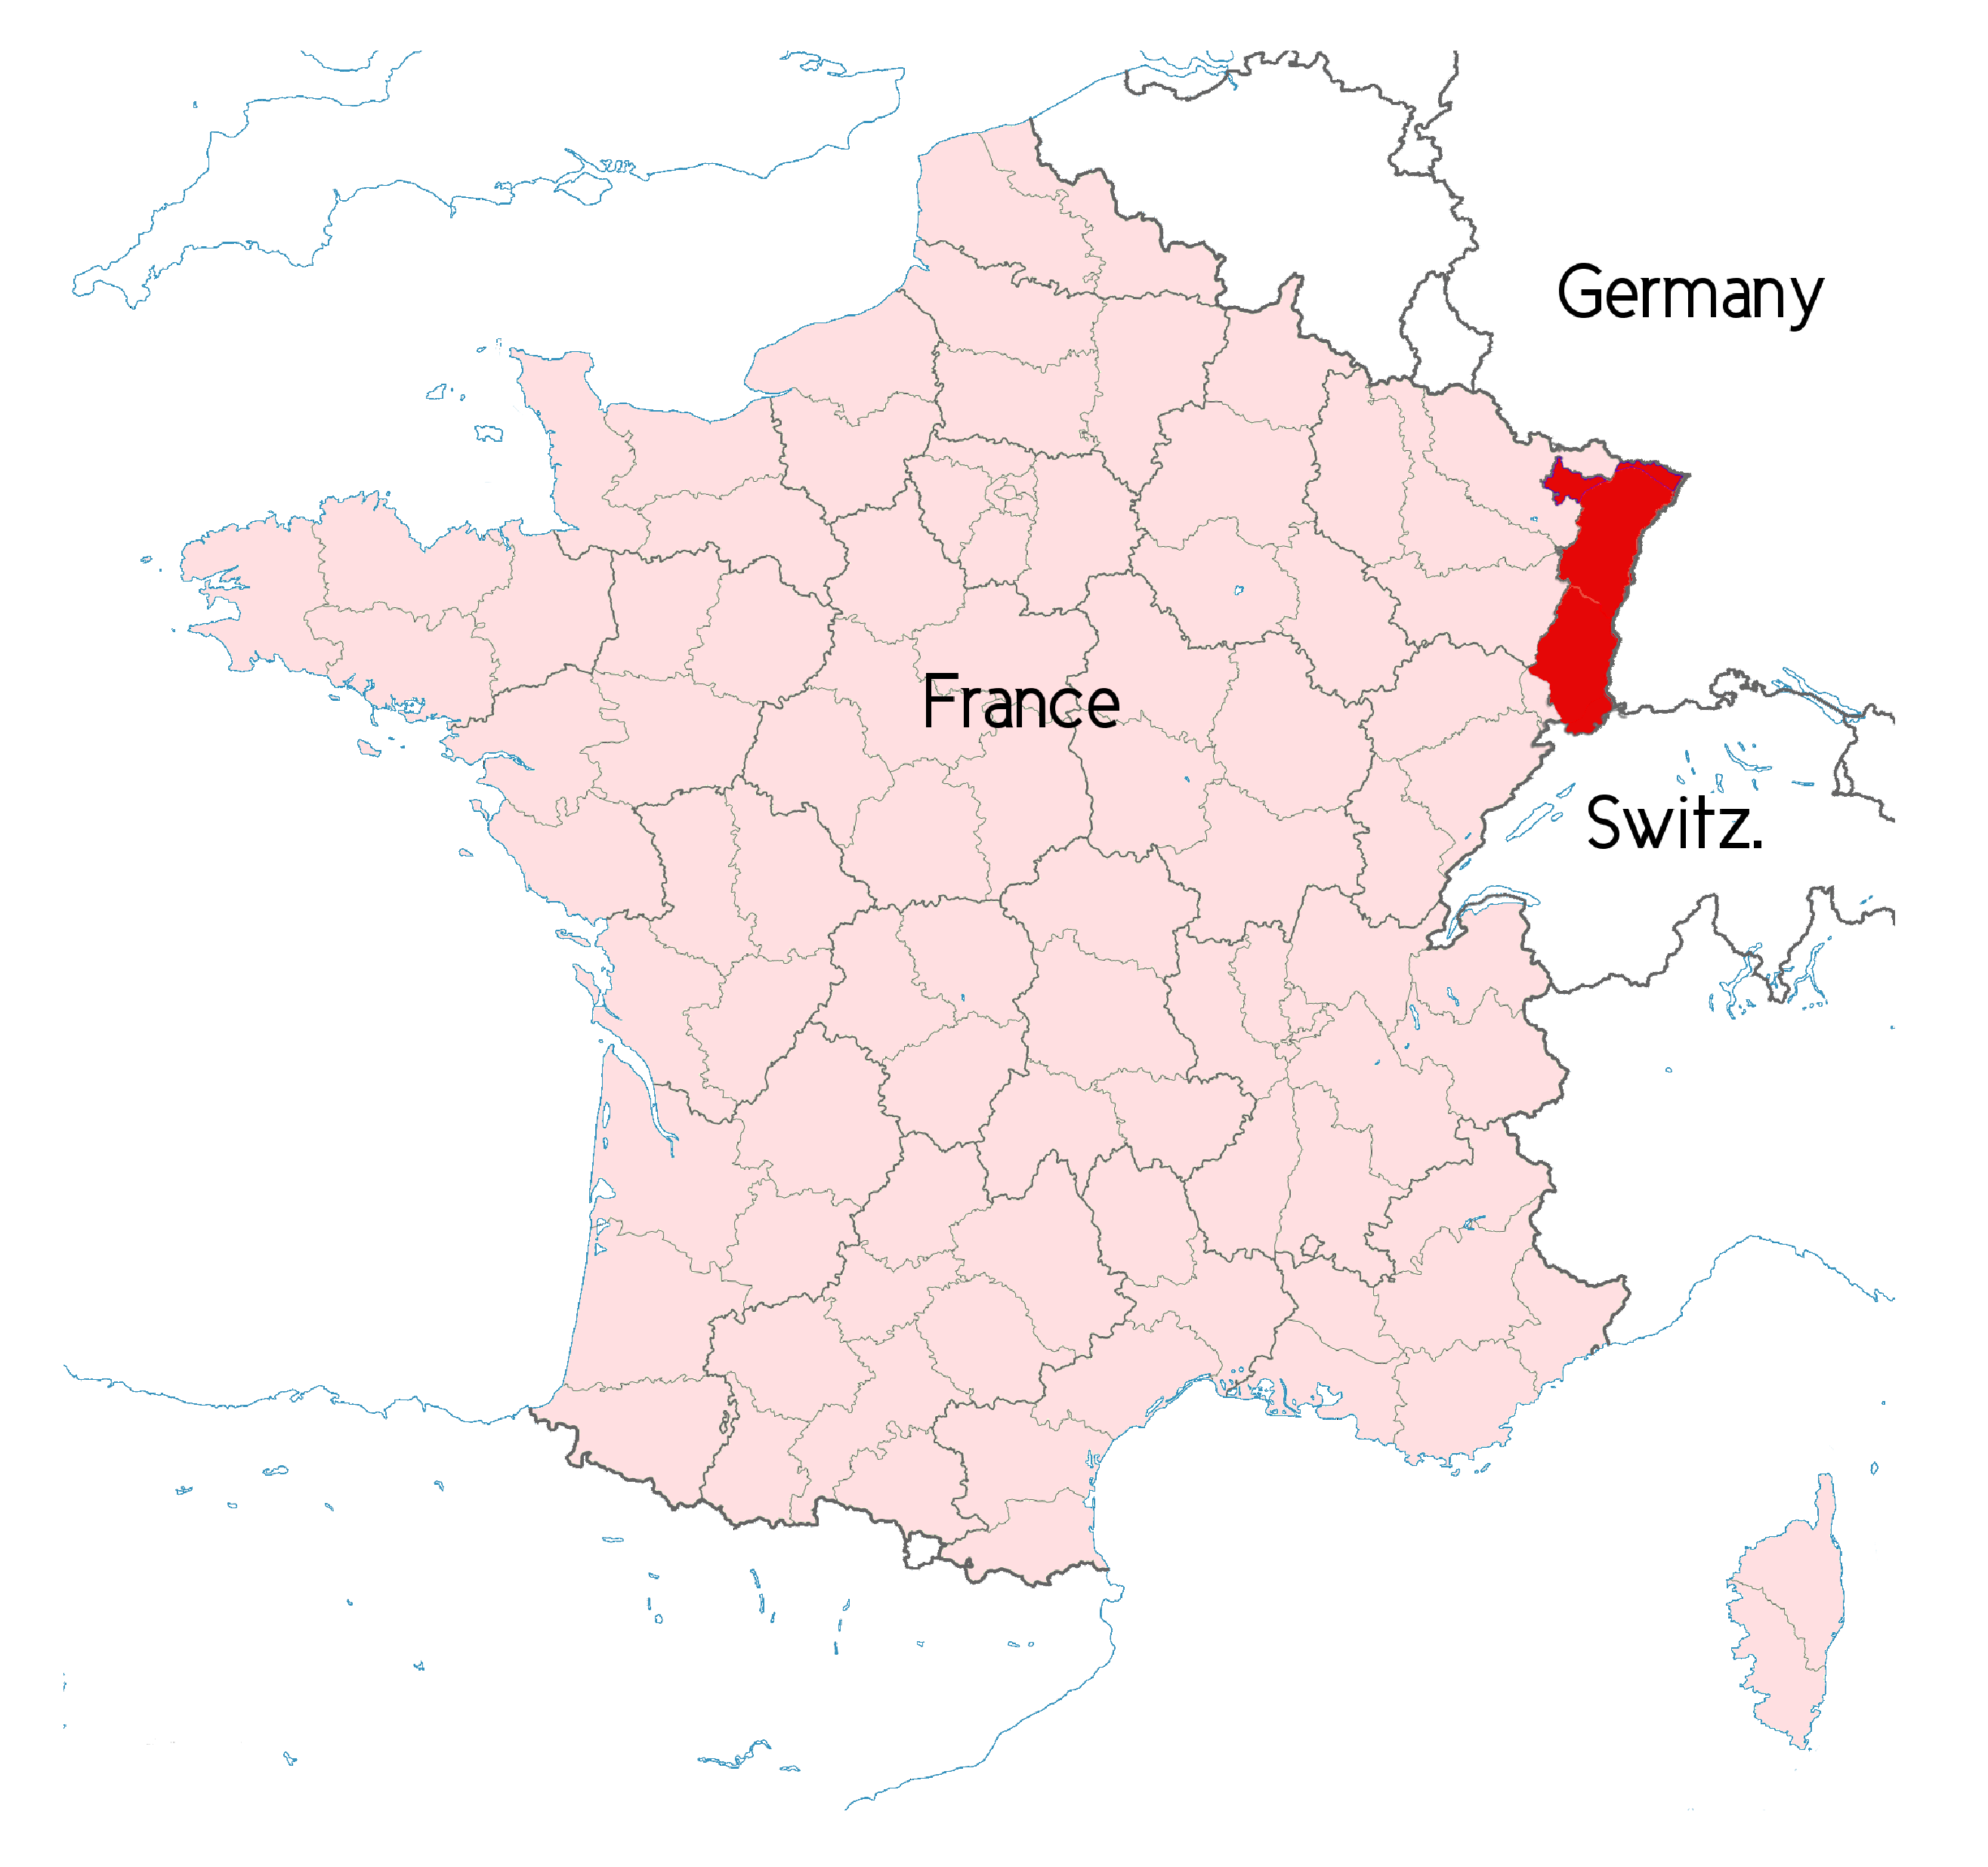
\includegraphics[width=1.2\textwidth]{figures/France-uni.png}};
        \end{tikzpicture}
      \end{column}
      \begin{column}{0.6\textwidth}
        \begin{itemize}
        \item continuum de dialectes alémaniques
        \item \textbf{550,000 locuteurs} en 1999\footnotemark[1]
        \item population majoritairement bilingue
        \end{itemize}
      \end{column}
    \end{columns}    
    \footnotetext[1]{D'après \cite{institut_2004}.}
  }
\end{frame}

%% Le continuum

\begin{frame}{Le continuum dialectal}
  \begin{columns}
    \begin{column}{0.25\textwidth}
      \begin{tikzpicture}
        \node (img0) {\includegraphics[height=5.5cm]{figures/Elsass2.png}};
      \end{tikzpicture}
    \end{column}
    \begin{column}{0.85\textwidth}
      \small
      \textit{\textcolor{nla}{Mer müess mache dass d'Kerisch mittess im Dorf bliebt.} \\~\\ %(Alémanique du nord)
        \textcolor{nla}{Mer müess màche  dàss d'Kìrisch mìtel im Dorf blibt}.*\\~\\ % Alémanique du nord (graphie orthal)
        \textcolor{sla}{Mer müass màcha dàss d’Kîrch mittess îm Dorf blibt}.\\~\\ % (Alémanique du Sud (graphie GRIMAL))
        \textcolor{sla}{M'r müess màcha dàss d'Kìrch mìtel im Dorf blibt}.* \\~\\  % (Orthal - Sud)
      }
      \footnotesize *rédigé en graphie ORTHAL \footnotemark[1] \\~\\ 
      %\footnotesize (Nous devons garder l'église au centre du village.)
    \end{column}
  \end{columns}
  \begin{center}
    \normalsize
    \visible<2->{Malgré plusieurs propositions de standardisation, il n'existe \uline{\textbf{pas d'orthographe consensuelle à ce jour}}} 
  \end{center}
  \footnotetext[1]{Voir \cite{Zeidler2008}.}
\end{frame}

%%%% Alsacien et TAL
\subsection{Alsacien et traitement automatique des langues (TAL)}

%% LPD - niveaux
\begin{frame}{Niveaux d'analyse en traitement automatique des langues}
  \centering
  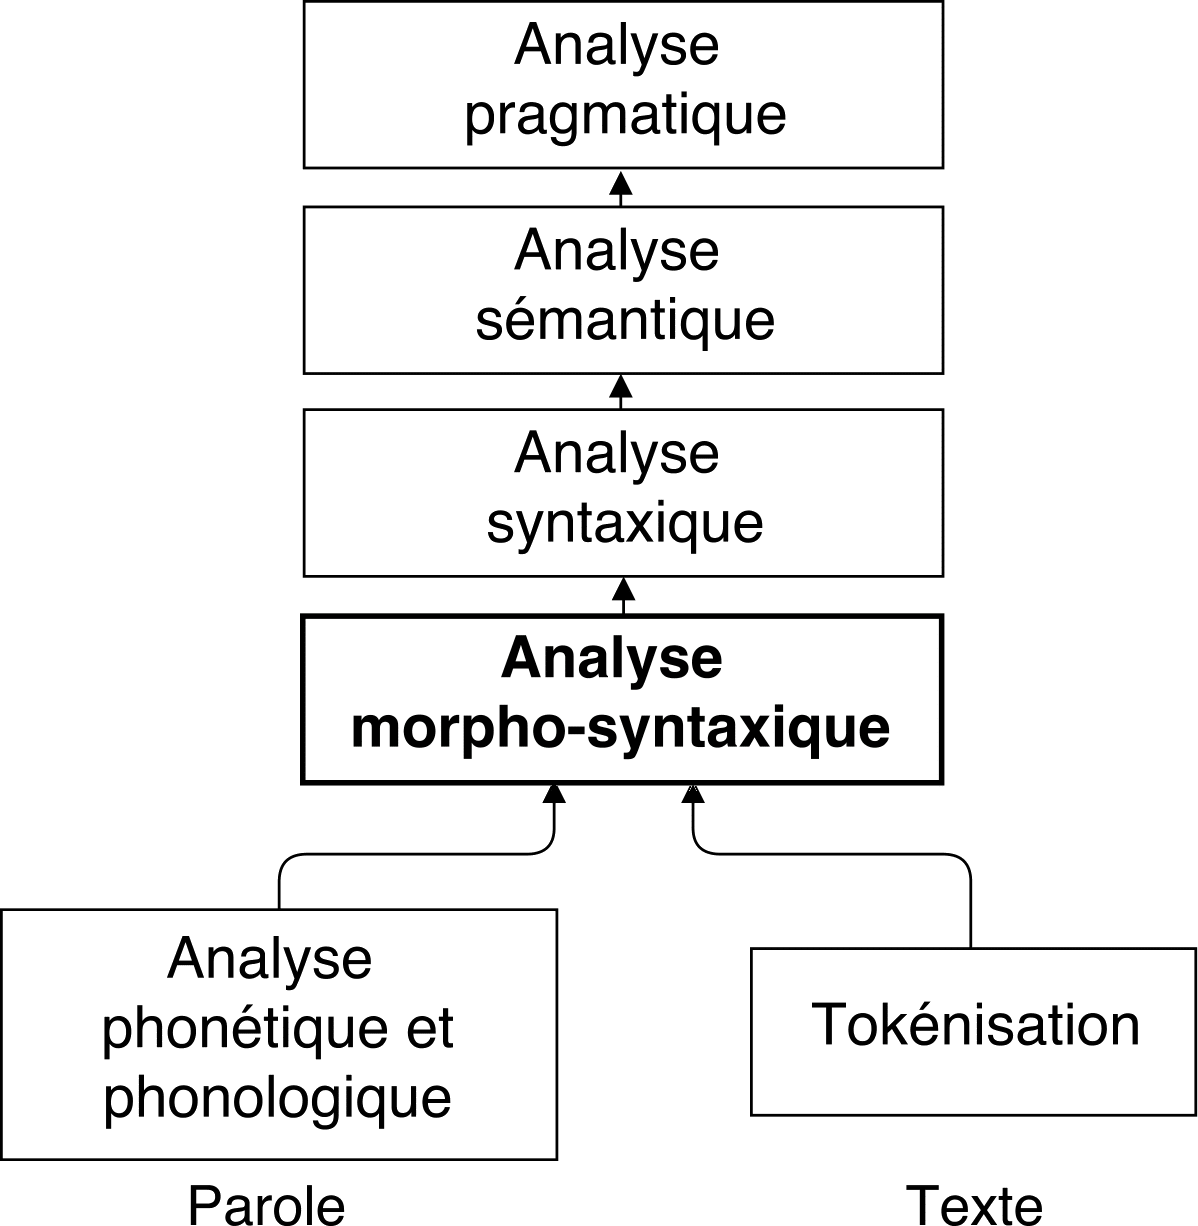
\includegraphics[scale=0.12]{figures/niveaux-0-trans.png}
\end{frame}

\begin{frame}{L'alsacien : une langue \og peu dotée \fg{} pour le TAL}
  \centering
  \small Outils existant pour le traitement automatique de l'alsacien :\\~\\~\\
  \begin{columns}
    \visible<2->{
      \begin{column}{0.4\textwidth}
        \centering
        \begin{itemize}
        \item un tokéniseur\footnotemark[1] :
        \end{itemize}
      \end{column}
      \begin{column}{0.6\textwidth}
        \begin{table}[]
          \centering
          
          %\resizebox{0.8\linewidth}{!}{
          \begin{tabular}{ccc}
            \toprule
            \multicolumn{3}{c}{\textit{\textbf{Ich mach’s}}}  \\ \hline
            \textit{\textbf{Ich}} & \textit{\textbf{mach}} & \textit{\textbf{’s}}\\
            \small \og je \fg{}   & \small \og fais \fg{}  & \small \og le \fg{}  \\ \toprule
          \end{tabular}
          %}
        \end{table}
        
      \end{column}
    }
  \end{columns}
  \footnotetext[1]{Fourni par Delphine Bernhard, LiLPa, Strasbourg.}
\end{frame}

\begin{frame}{L'alsacien : une langue \og peu dotée \fg{} pour le TAL}
  \centering
  \small Outils existant pour le traitement automatique de l'alsacien :\\
  \begin{itemize}
\item un tokéniseur\footnotemark[1]
    \visible{\item  \tool{Stanford POS Tagger}\\~\cite{Toutanova2003}\footnotemark[2]}
    \visible<2->{\item \tool{MElt}~\cite{Denis2010}, \\ entraîné régulièrement avec nos
\visible<3->{\smash{\raisebox{3\dimexpr0.3\baselineskip-5\itemsep+5.5\parskip}{$\left.\rule{0pt}{2.3\dimexpr1\baselineskip+2\itemsep-1\parskip}\right\}$\ \parbox{2.8cm}{\center utilisés comme \\ \textbf{outils de pré-annotation}}}}}
      \\ données annotées (\tool{MElt$_{ALS}$})}\\
  \end{itemize}
  \bigskip
  \visible<3->{
    \Wider[4em]{
      \begin{table}[]
        \centering
        \resizebox{\linewidth}{!}{
          \begin{tabular}{p{3cm}|cccccccccccc}
            \toprule  
            & \textit{\textbf{Ùf}} & \textit{\textbf{e}}                 & \textit{\textbf{Grìeni-Lìnse}}       & \textit{\textbf{Bett}}               & \textit{\textbf{leje}}               & \textit{\textbf{ùn}}                 & \textit{\textbf{d'}}                & \textit{\textbf{Sauce}}              & \textit{\textbf{drùm}}              & \textit{\textbf{erùm}}              & \textit{\textbf{nàppìere}}    & \textit{\textbf{.}}           \\  \hline
            \tool{Stanford Tagger}   &  {\color{red}\textsc{x}}           & {\color{mylightgreen} \textbf{\textsc{det}}} & {\color{mylightgreen} \textbf{\textsc{noun}}} & {\color{mylightgreen} \textbf{\textsc{noun}}} & {\color{mylightgreen} \textbf{\textsc{verb}}} & {\color{mylightgreen} \textbf{\textsc{conj}}} & {\color{mylightgreen} \textbf{\textsc{det}}} & {\color{mylightgreen} \textbf{\textsc{noun}}} &  {\color{red}\textsc{pron}}                       & {\color{mylightgreen} \textbf{\textsc{adp}}} & {\color{mylightgreen} \textbf{\textsc{verb}}} & {\color{mylightgreen} \textbf{\textsc{punct}}} \\
            \tool{MElt$_{ALS}$} &  {\color{red}\textsc{propn}}       &  {\color{red}\textsc{verb}}                       &  {\color{red}\textsc{adj}}                         & {\color{mylightgreen} \textbf{\textsc{noun}}} &  {\color{red}\textsc{propn}}                       & {\color{mylightgreen} \textbf{\textsc{conj}}} & {\color{mylightgreen} \textbf{\textsc{det}}} & {\color{mylightgreen} \textbf{\textsc{noun}}} & {\color{mylightgreen} \textbf{\textsc{adv}}} & {\color{mylightgreen} \textbf{\textsc{adp}}} & {\color{mylightgreen} \textbf{\textsc{verb}}}& {\color{mylightgreen} \textbf{\textsc{punct}}}
            %% \\ \hline \hline 
            %% Annotation correcte & \textsc{adp}         & \textsc{det}                        & \textsc{noun}                        & \textsc{noun}                        & \textsc{verb}                        & \textsc{conj}                        & \textsc{det}                        & \textsc{noun}                        & \textsc{adv}                        & \textsc{adp}                        & \textsc{verb}             & {\color{mylightgreen} \textsc{punct}}
            \\ \toprule            

          \end{tabular}
        }
      \end{table}
    }
  }
  %% \begin{column}{0.46\textwidth}
  %%   \visible<3->{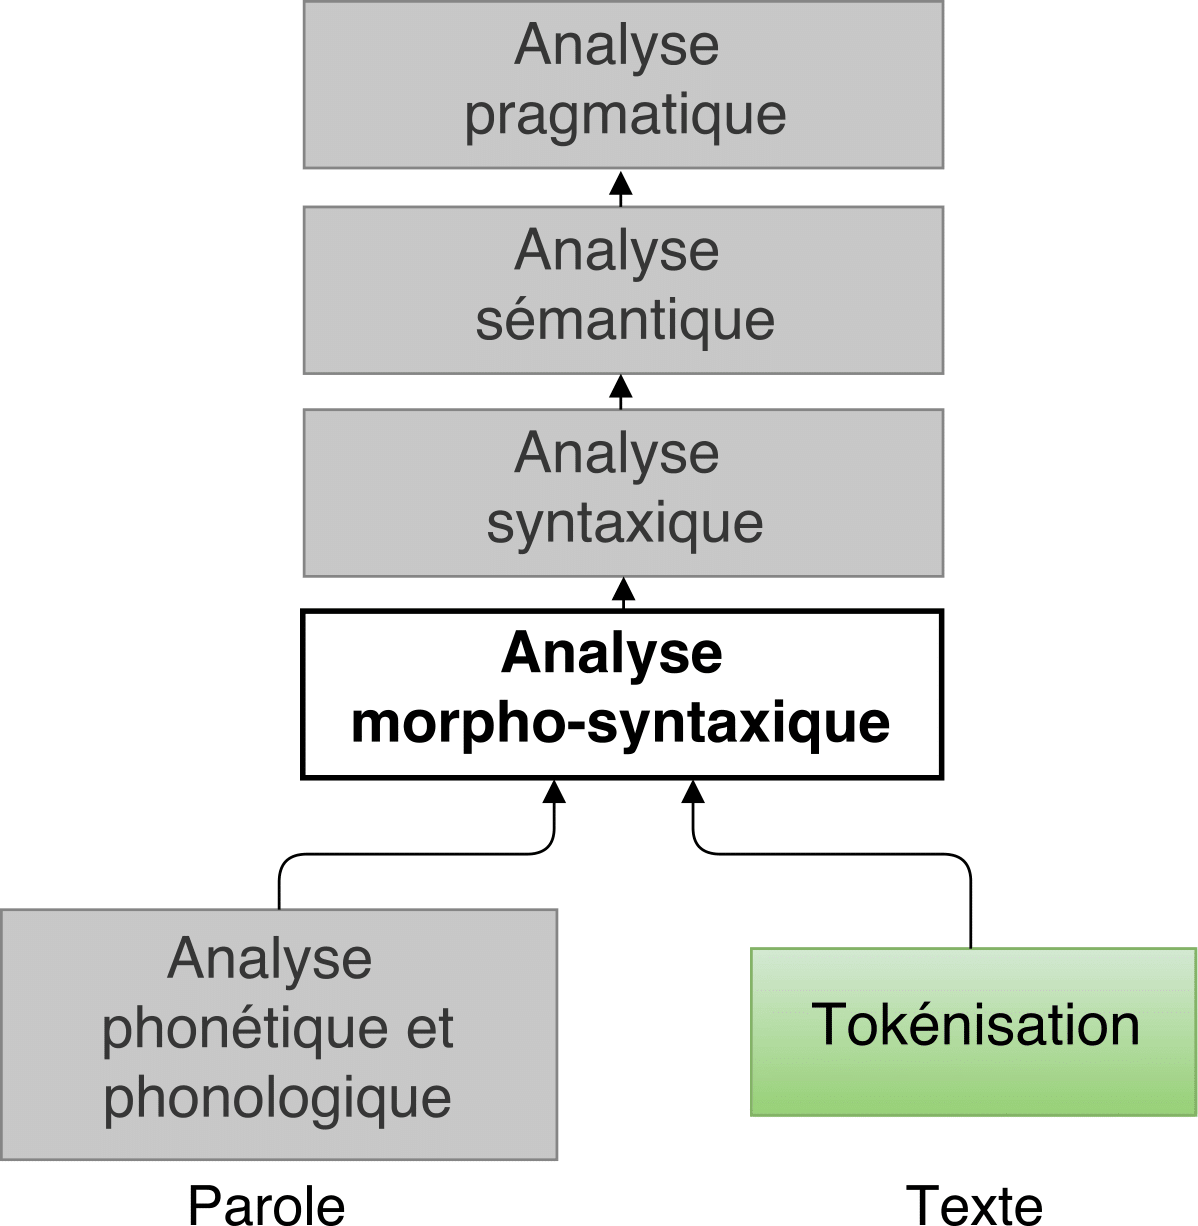
\includegraphics[width=0.8\linewidth]{figures/niveaux-trans.png}}
  %% \end{column}
  \footnotetext[1]{Fourni par Delphine Bernhard, LiLPa, Strasbourg.}
  \footnotetext[2]{Utilisé selon la méthodologie décrite par \cite{bernhard_es_2013}.}
\end{frame}

%% Apprentissage
\begin{frame}{\small La création d'outils de TAL \textit{via} l'apprentissage automatique}
  
\centering
  les corpus annotés sont nécessaires pour \textbf{entraîner} et \textbf{évaluer} les outils automatiques d'annotation \\~\\
  \Wider[3em]{
    \begin{figure}
  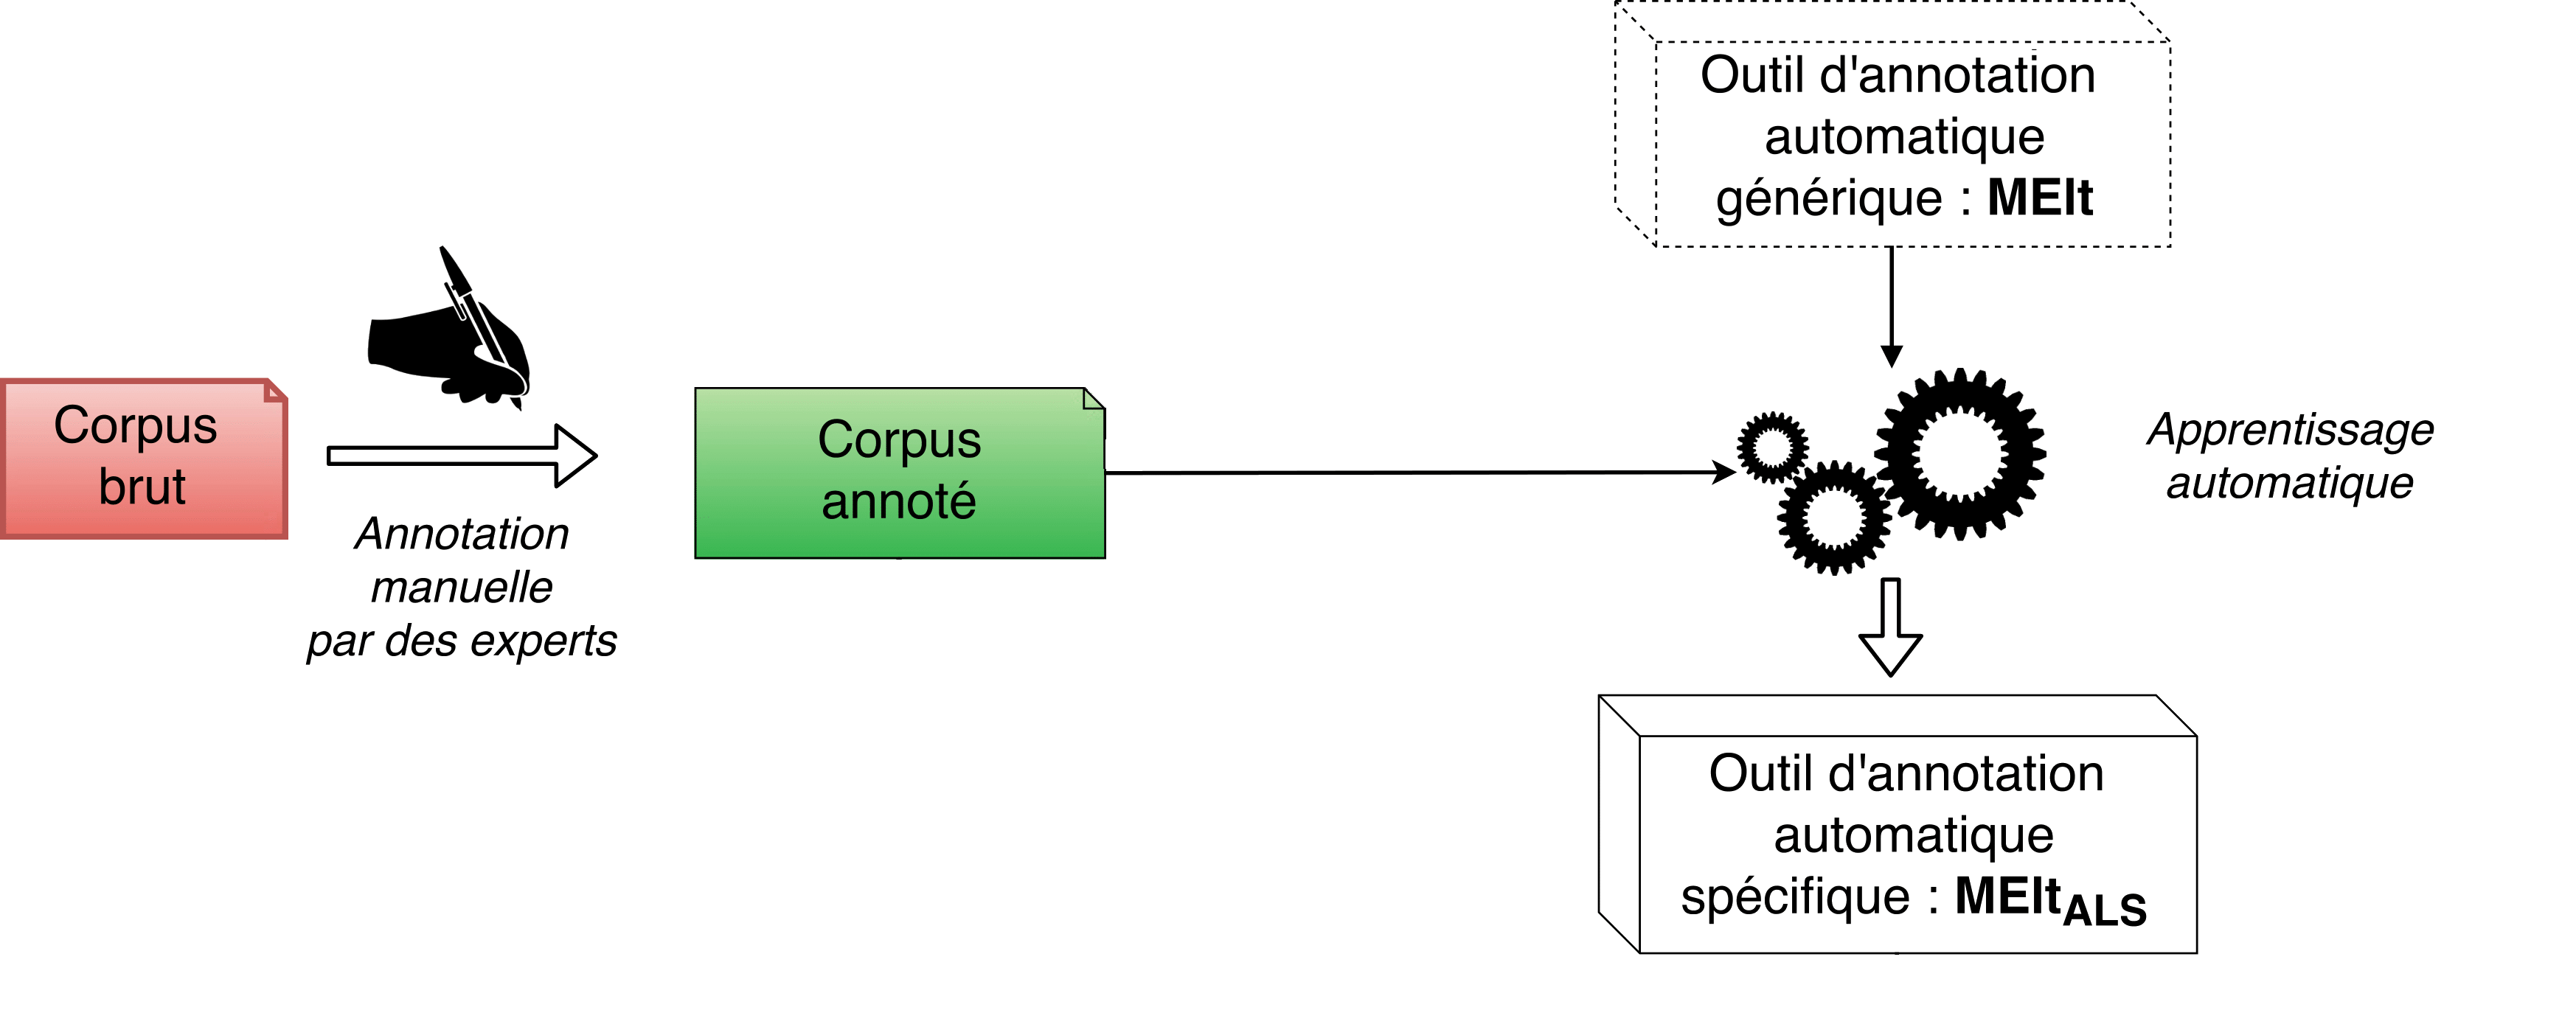
\includegraphics[width=0.8\linewidth]{figures/annotation-experts-0.png} 
  \end{figure}
    \hfill\cite{Fort2012} \\
    \centering
  \visible<2->{l'annotation manuelle \og classique \fg{} est un processus \textbf{long} et \textbf{coûteux} \\
  \scriptsize par exemple, la construction du \tool{Prague Treebank} en 5 ans a été évaluée à 600~000 \$ par~\cite{Bohmova2001}}
}
\end{frame} 


\begin{frame}{Notre objectif}
  \centering
  pallier le manque de ressources humaines et financières
  \begin{center}
    $\rightarrow$ permettre aux \textbf{locuteurs de l'alsacien} de participer \textbf{collaborativement} à l'annotation d'un corpus \\ \textit{via} une plate-forme dédiée \\~\\
    \visible<2->{$\rightarrow$ mettre en place une \textbf{méthodologie d'évaluation} de l'annotation assurant la qualité des corpus produits}
  \end{center}
\end{frame}

\subsection{Ressources initiales et annotation collaborative de corpus}
%% POS
\begin{frame}{Jeu d'étiquettes utilisé}
  \begin{table}[!ht]
    \centering
    \resizebox{0.7\linewidth}{!}{
      \begin{tabular}{ccccc}
        \toprule
        \textsc{adj} & \textsc{adp} &  \textsc{adv} & \textsc{aux} & \textsc{conj} \\
        \textsc{det} & \textsc{sconj} & \textsc{intj} &  \textsc{noun}  &  \textsc{num} \\
         \textsc{part} & \textsc{pron} & \textsc{propn} & \textsc{punct }& \textsc{sconj} \\
         & \textsc{sym} &   \textsc{verb} &  \textsc{x}&  \\
         \toprule  
      \end{tabular}
    }
  \end{table}
  \centering
   
    17 catégories\footnotemark[1]
  \footnotetext[1]{Voir \url{http://universaldependencies.org/u/pos/all.html},\\ \cite{petrov2011universal}.}
\end{frame}
% c'est le jeu d'étiquette qui a été utilisé dans les ressources de départ dont nous avons pu tirer parti
%% CI : ressources
\begin{frame}{Conditions initiales : les ressources - lexiques}
  \Wider[2.5em]{
    \begin{itemize}
    \item     un lexique de 322 mots fréquents ($L_{MO}$) ~\cite{bernhard_es_2013}
    \item     un lexique compilé depuis différentes sources de 40~000 entrées ($L_{gsw}$) telles que \\
      
    \end{itemize}
    \begin{table}[]
      \centering
      \resizebox{0.35\linewidth}{!}{
        \begin{tabular}{ll}
          \textit{\textbf{Elleböje}}  & \textsc{noun} \\
          \textit{\textbf{Ellaboja}}  & \textsc{noun} \\
          \textit{\textbf{Elleboje}}  & \textsc{noun} \\
          \textit{\textbf{Ällabooga}} & \textsc{noun} \\ \toprule
          \multicolumn{2}{c}{pour le mot \og coude \fg{}} 
        \end{tabular}
      }
    \end{table}
  }
  %% \visible<2->{
    %%   \begin{table}[]
    %%     \centering
    %%     \small	
    %%     \begin{tabular}{l|l|c|c}
    %%       \toprule
    %%       & Source & \multicolumn{2}{l}{Nb. mots} \\ \hline
    %%       \multicolumn{1}{l|}{\multirow{3}{*}{\pbox{2
    %%             cm}{Corpus de \\référence}}} & \multirow{2}{*} \nla\tool{Wikipédia} & {875} & \multirow{3}{*}{1.468} \\\cline{2-3} 
    %%         \multicolumn{1}{l|}{} & \sla Recette de cuisine  & 362 &  \\ \cline{2-3} 
    %%         \multicolumn{1}{l|}{} & \sla Pièce de théâtre
    %%         & 231 & \pause \\ \hline \hline 
    %%         \multicolumn{1}{l|}{Corpus Brut} & \nla \tool{Wikipédia}  & \multicolumn{2}{c}{8.833 (65\% annoté)} \\ \toprule  
    %%       \end{tabular}
    %%     \end{table}
    %% }
\end{frame}


\begin{frame}{Conditions initiales : les ressources - corpus} 
  \begin{itemize}
  \item \small  \textbf{un corpus annoté de référence}\footnotemark[1] utilisé pour former les participants et évaluer notre système  (102 phrases) \\
    \vspace{-0.3cm}
    \begin{table}[]
      \centering
      \resizebox{\linewidth}{!}{
        \begin{tabular}{ccccccccc}
          \toprule
          \textit{\textbf{D'}} & \textit{\textbf{grìene}} & \textit{\textbf{Lìnse}} & \textit{\textbf{12}} & \textit{\textbf{Stùnde}} & \textit{\textbf{làng}} & \textit{\textbf{inweiche}} & \textit{\textbf{lon}} & \textit{\textbf{.}} \\
          \textsc{det} & \textsc{adj} & \textsc{noun}  & \textsc{num} & \textsc{noun}   & \textsc{adv}  & \textsc{verb}     & \textsc{verb} & \textsc{punct} \\ \toprule
        \end{tabular}
      }
    \end{table}
    
    \visible<2->{
    \item \small \textbf{un corpus brut} issu de la Wikipédia alémanique\footnotemark[2] 
    }
  \end{itemize}
  \vspace{-0.2cm}
  \begin{columns}
    \begin{column}{0.2\textwidth}
      \begin{tikzpicture}
        \node (img0) {\includegraphics[height=4.1cm]{figures/Elsass2.png}};
      \end{tikzpicture}
    \end{column}
    \begin{column}{0.8\textwidth}
      \begin{table}[]
        \centering
        \small
        \resizebox{1\linewidth}{!}{
        \begin{tabular}{l|l|c|c}
          \toprule
          & Source & \multicolumn{2}{p{3cm}}{Nb. tokens} \\ \hline
          \multicolumn{1}{l|}{\multirow{3}{*}{\pbox{2cm}{Corpus de \\référence}}} & \multirow{2}{*} \nla\tool{Wikipédia} & {875} & \multirow{3}{*}{1~468} \\\cline{2-3} 
          \multicolumn{1}{l|}{} & \sla Recette de cuisine  & 362 &  \\ \cline{2-3} 
          \multicolumn{1}{l|}{} & \sla Pièce de théâtre
          & 231 & \pause \\ \hline \hline 
          \multicolumn{1}{l|}{Corpus brut} & \nla \tool{Wikipédia}  & \multicolumn{2}{c}{8~833} \\ \toprule  
        \end{tabular}
        }
      \end{table}
    \end{column}
  \end{columns}
  \tiny\footnotetext[1]{\tiny Par Delphine Bernhard et Lucie Steiblé, LiLPa, Strasbourg.}
  \footnotetext[2]{\tiny Voir : http///als.wikipedia.org.}
\end{frame}

%% CI : outilsx
%\begin{frame}{Conditions initiales : les outils existants}
%%   \begin{enumerate}
%%   \item German \tool{TreeTagger}~\cite{Schmid1997}\footnote{Utilisé selon la méthodologie décrite par \cite{bernhard_es_2013}}
%%     \smash{\raisebox{1.8\dimexpr0.3\baselineskip-6.3\itemsep+5.5\parskip}{$\left.\rule{0pt}{1.5\dimexpr1\baselineskip+2\itemsep-1\parskip}\right\}$\ \parbox{2.8cm}{\center utilisés comme \\ \textbf{outils de pré-annotation}}}}  
%%   \item \tool{MElt}~\cite{Denis2010}, \\ entraîné régulièrement avec nos \\ données annotées (\tool{MElt$_{ALS}$})\\
%%   \end{enumerate}
%%   \bigskip
%%   \Wider[4em]{
%%   \begin{table}[]
%%     \centering
%%       \resizebox{\linewidth}{!}{
%%         \begin{tabular}{p{2cm}|cccccccccccc}
%%           \toprule  
%%                          & \textit{\textbf{Ùf}} & \textit{\textbf{e}}                 & \textit{\textbf{Grìeni-Lìnse}}       & \textit{\textbf{Bett}}               & \textit{\textbf{leje}}               & \textit{\textbf{ùn}}                 & \textit{\textbf{d'}}                & \textit{\textbf{Sauce}}              & \textit{\textbf{drùm}}              & \textit{\textbf{erùm}}              & \textit{\textbf{nàppìere}}    & \textit{\textbf{.}}           \\  \hline
%% \tool{Treetagger}   &  {\color{red}\textsc{x}}           & {\color{mylightgreen} \textbf{\textsc{det}}} & {\color{mylightgreen} \textbf{\textsc{noun}}} & {\color{mylightgreen} \textbf{\textsc{noun}}} & {\color{mylightgreen} \textbf{\textsc{verb}}} & {\color{mylightgreen} \textbf{\textsc{conj}}} & {\color{mylightgreen} \textbf{\textsc{det}}} & {\color{mylightgreen} \textbf{\textsc{noun}}} &  {\color{red}\textsc{pron}}                       & {\color{mylightgreen} \textbf{\textsc{adp}}} & {\color{mylightgreen} \textbf{\textsc{verb}}} & {\color{mylightgreen} \textbf{\textsc{punct}}} \\
%% \tool{MElt$_{ALS}$} &  {\color{red}\textsc{propn}}       &  {\color{red}\textsc{verb}}                       &  {\color{red}\textsc{adj}}                         & {\color{mylightgreen} \textbf{\textsc{noun}}} &  {\color{red}\textsc{propn}}                       & {\color{mylightgreen} \textbf{\textsc{conj}}} & {\color{mylightgreen} \textbf{\textsc{det}}} & {\color{mylightgreen} \textbf{\textsc{noun}}} & {\color{mylightgreen} \textbf{\textsc{adv}}} & {\color{mylightgreen} \textbf{\textsc{adp}}} & {\color{mylightgreen} \textbf{\textsc{verb}}}& {\color{mylightgreen} \textbf{\textsc{punct}}}
%% %% \\ \hline \hline 
%% %% Annotation correcte & \textsc{adp}         & \textsc{det}                        & \textsc{noun}                        & \textsc{noun}                        & \textsc{verb}                        & \textsc{conj}                        & \textsc{det}                        & \textsc{noun}                        & \textsc{adv}                        & \textsc{adp}                        & \textsc{verb}             & {\color{mylightgreen} \textsc{punct}}
%% \\ \toprule            

%%     \end{tabular}
%%     }
%%   \end{table}
%%   }
%\end{frame}


\begin{frame}{L'annotation collaborative avec \tool{Bisame}}
  \begin{center}
    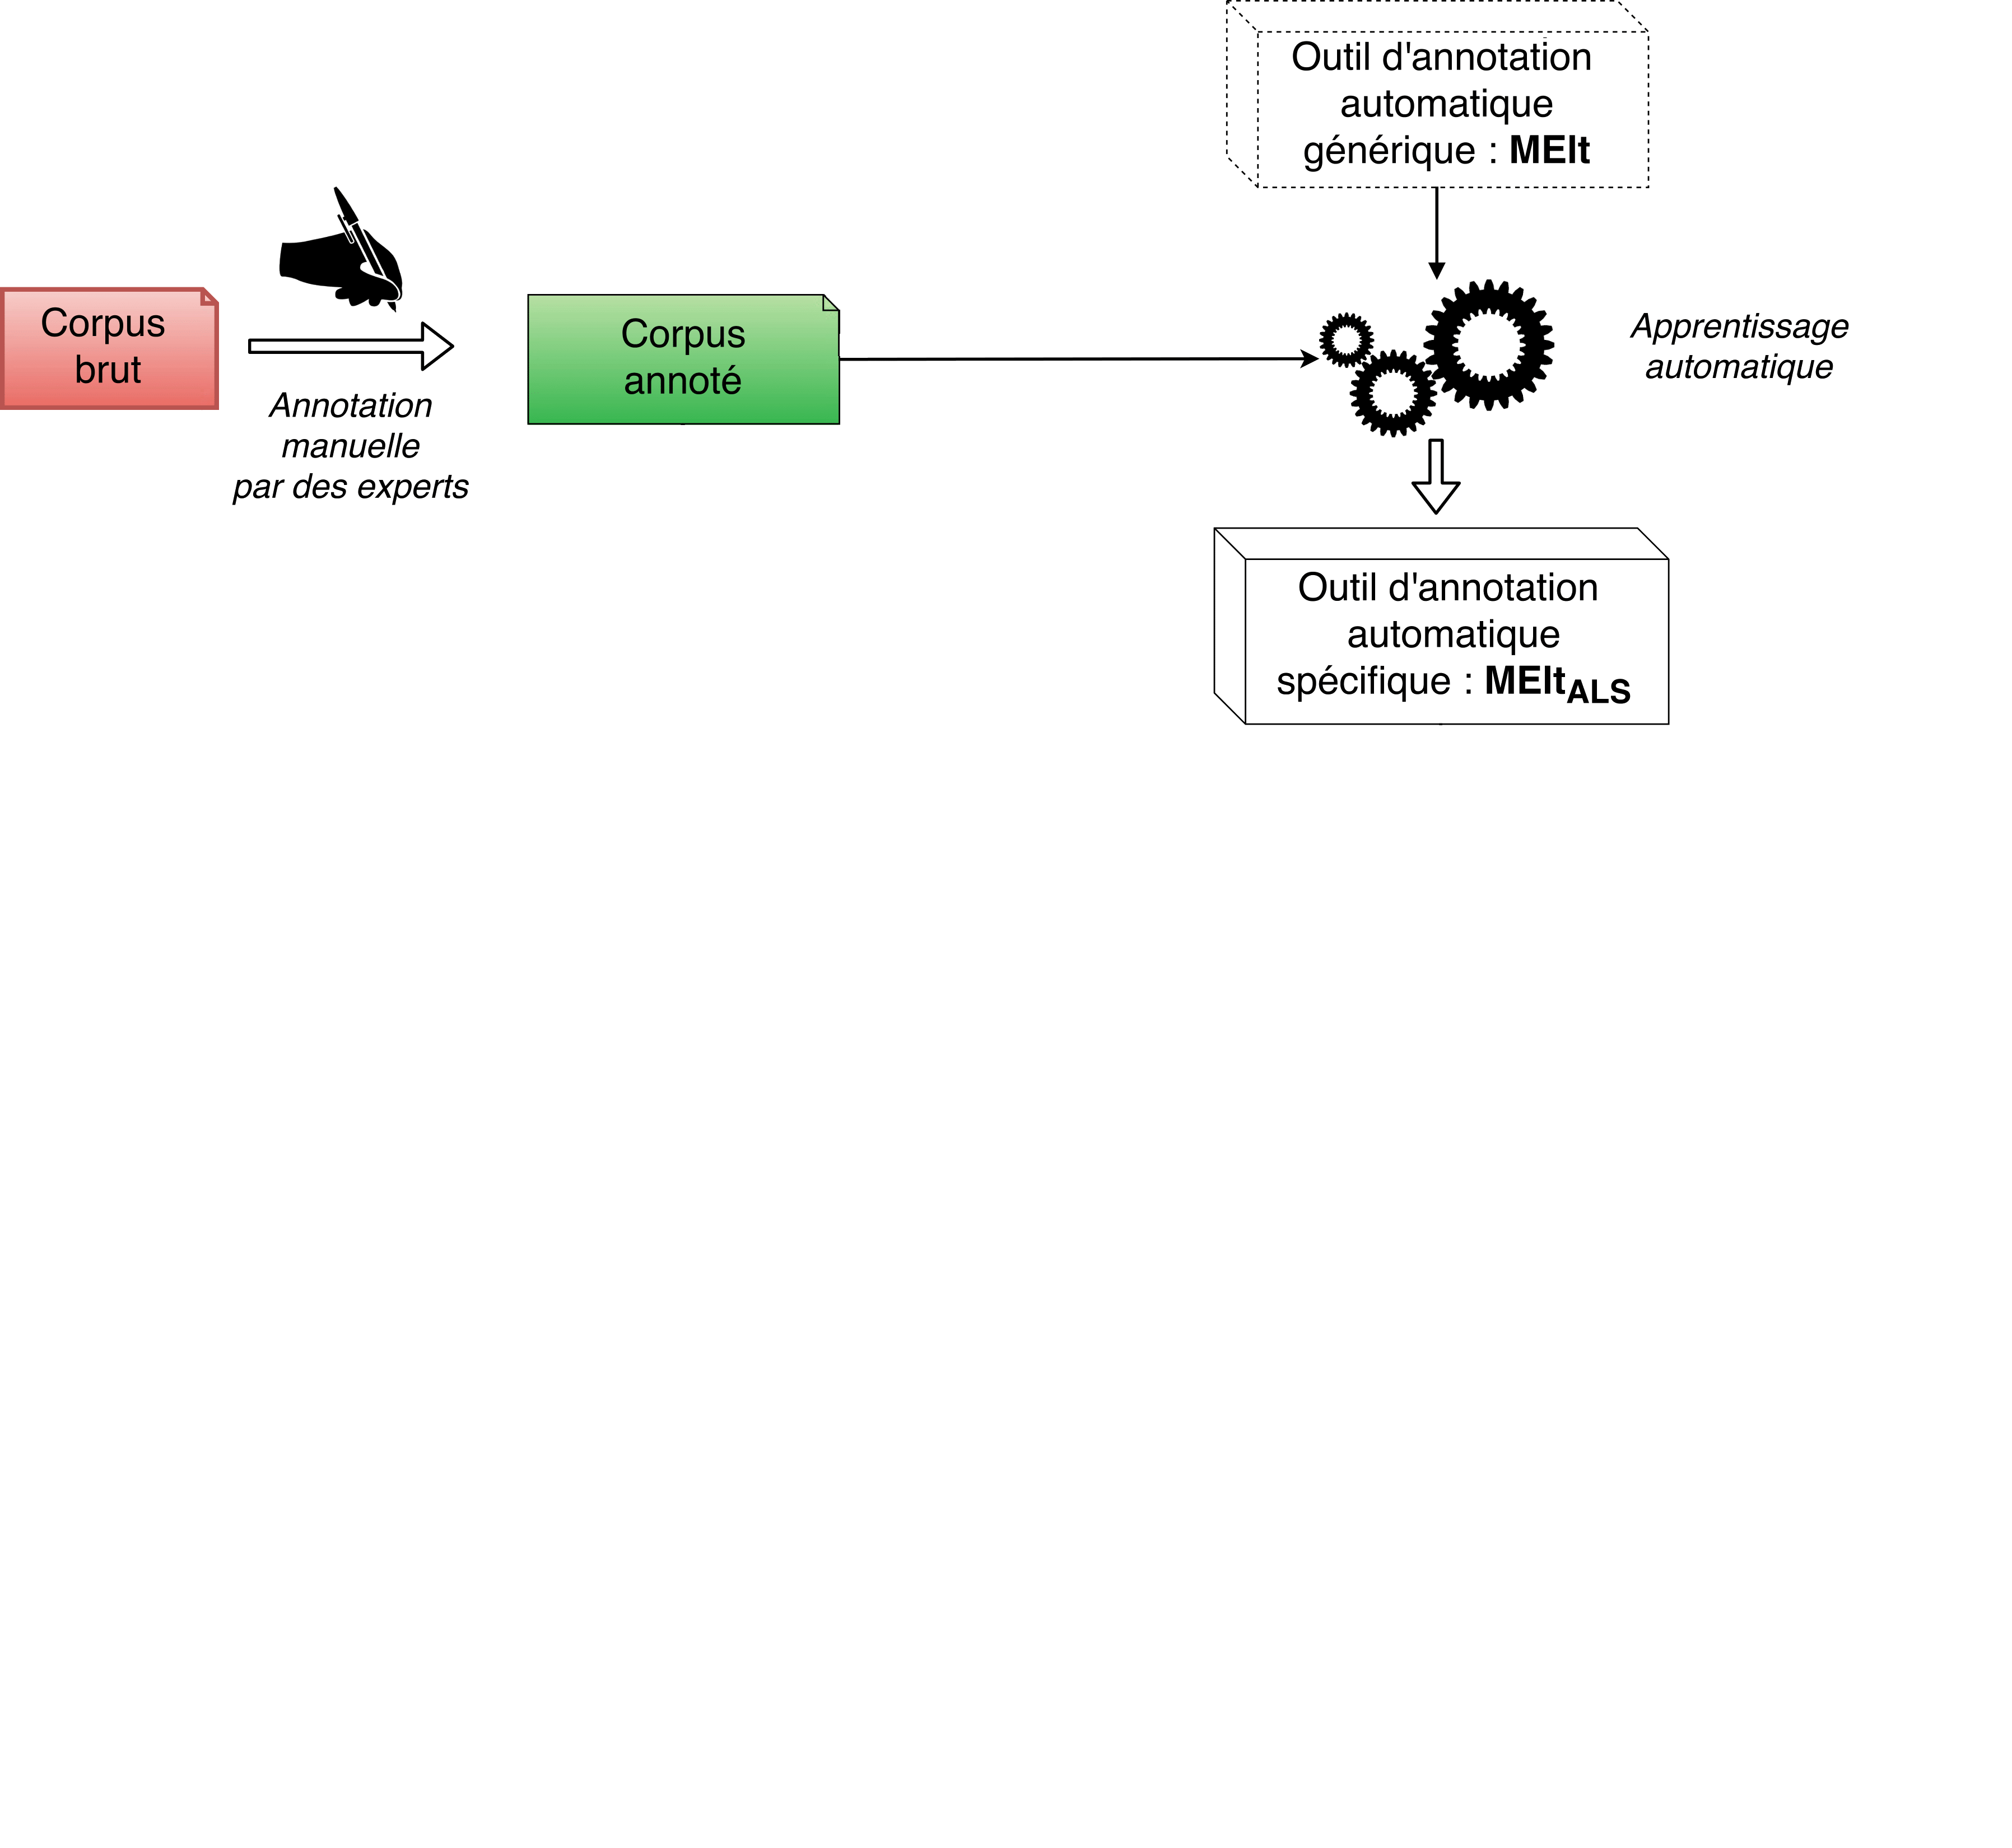
\includegraphics[width=0.8\linewidth]{figures/annotation-experts.png}
  \end{center}
    \hfill\cite{Fort2012} 
\end{frame}

\begin{frame}{L'annotation collaborative avec \tool{Bisame}}
  \begin{center}
    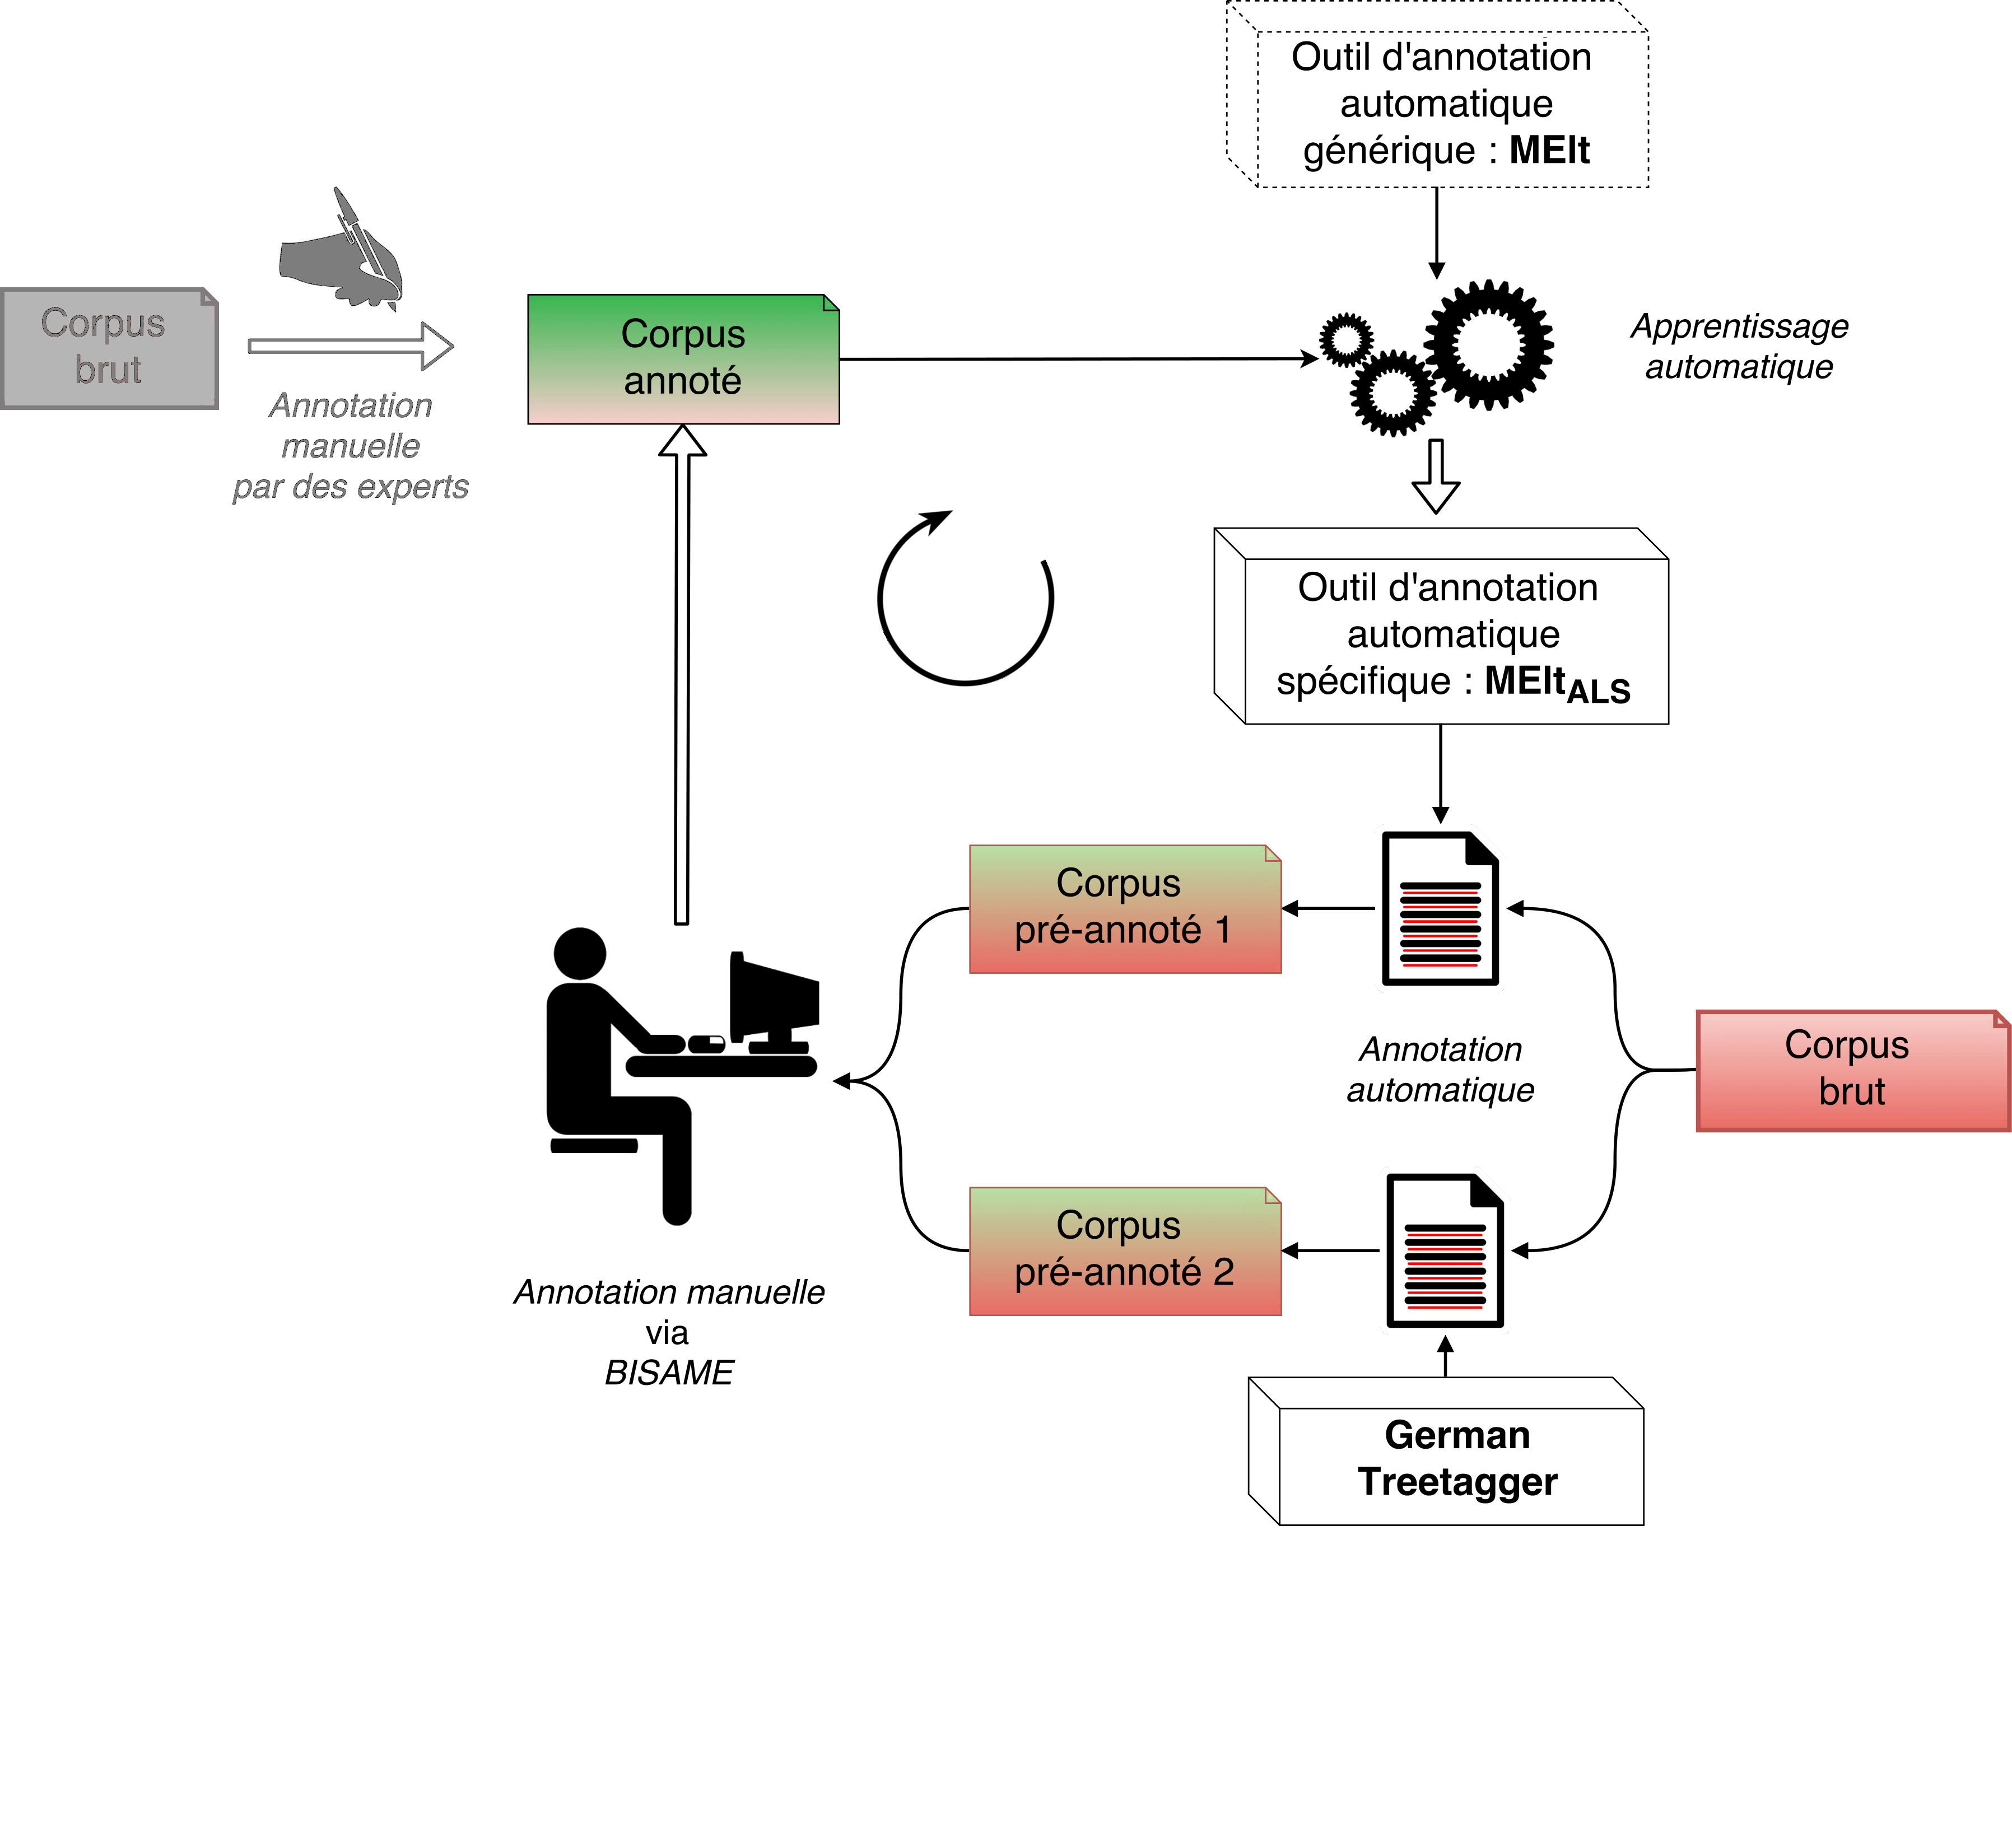
\includegraphics[width=0.8\linewidth]{figures/annotation-bisame-ref-1.png}
  \end{center}
  \hfill\cite{Fort2012}
\end{frame}


\begin{frame}{L'annotation collaborative avec \tool{Bisame}}
  \begin{center}
    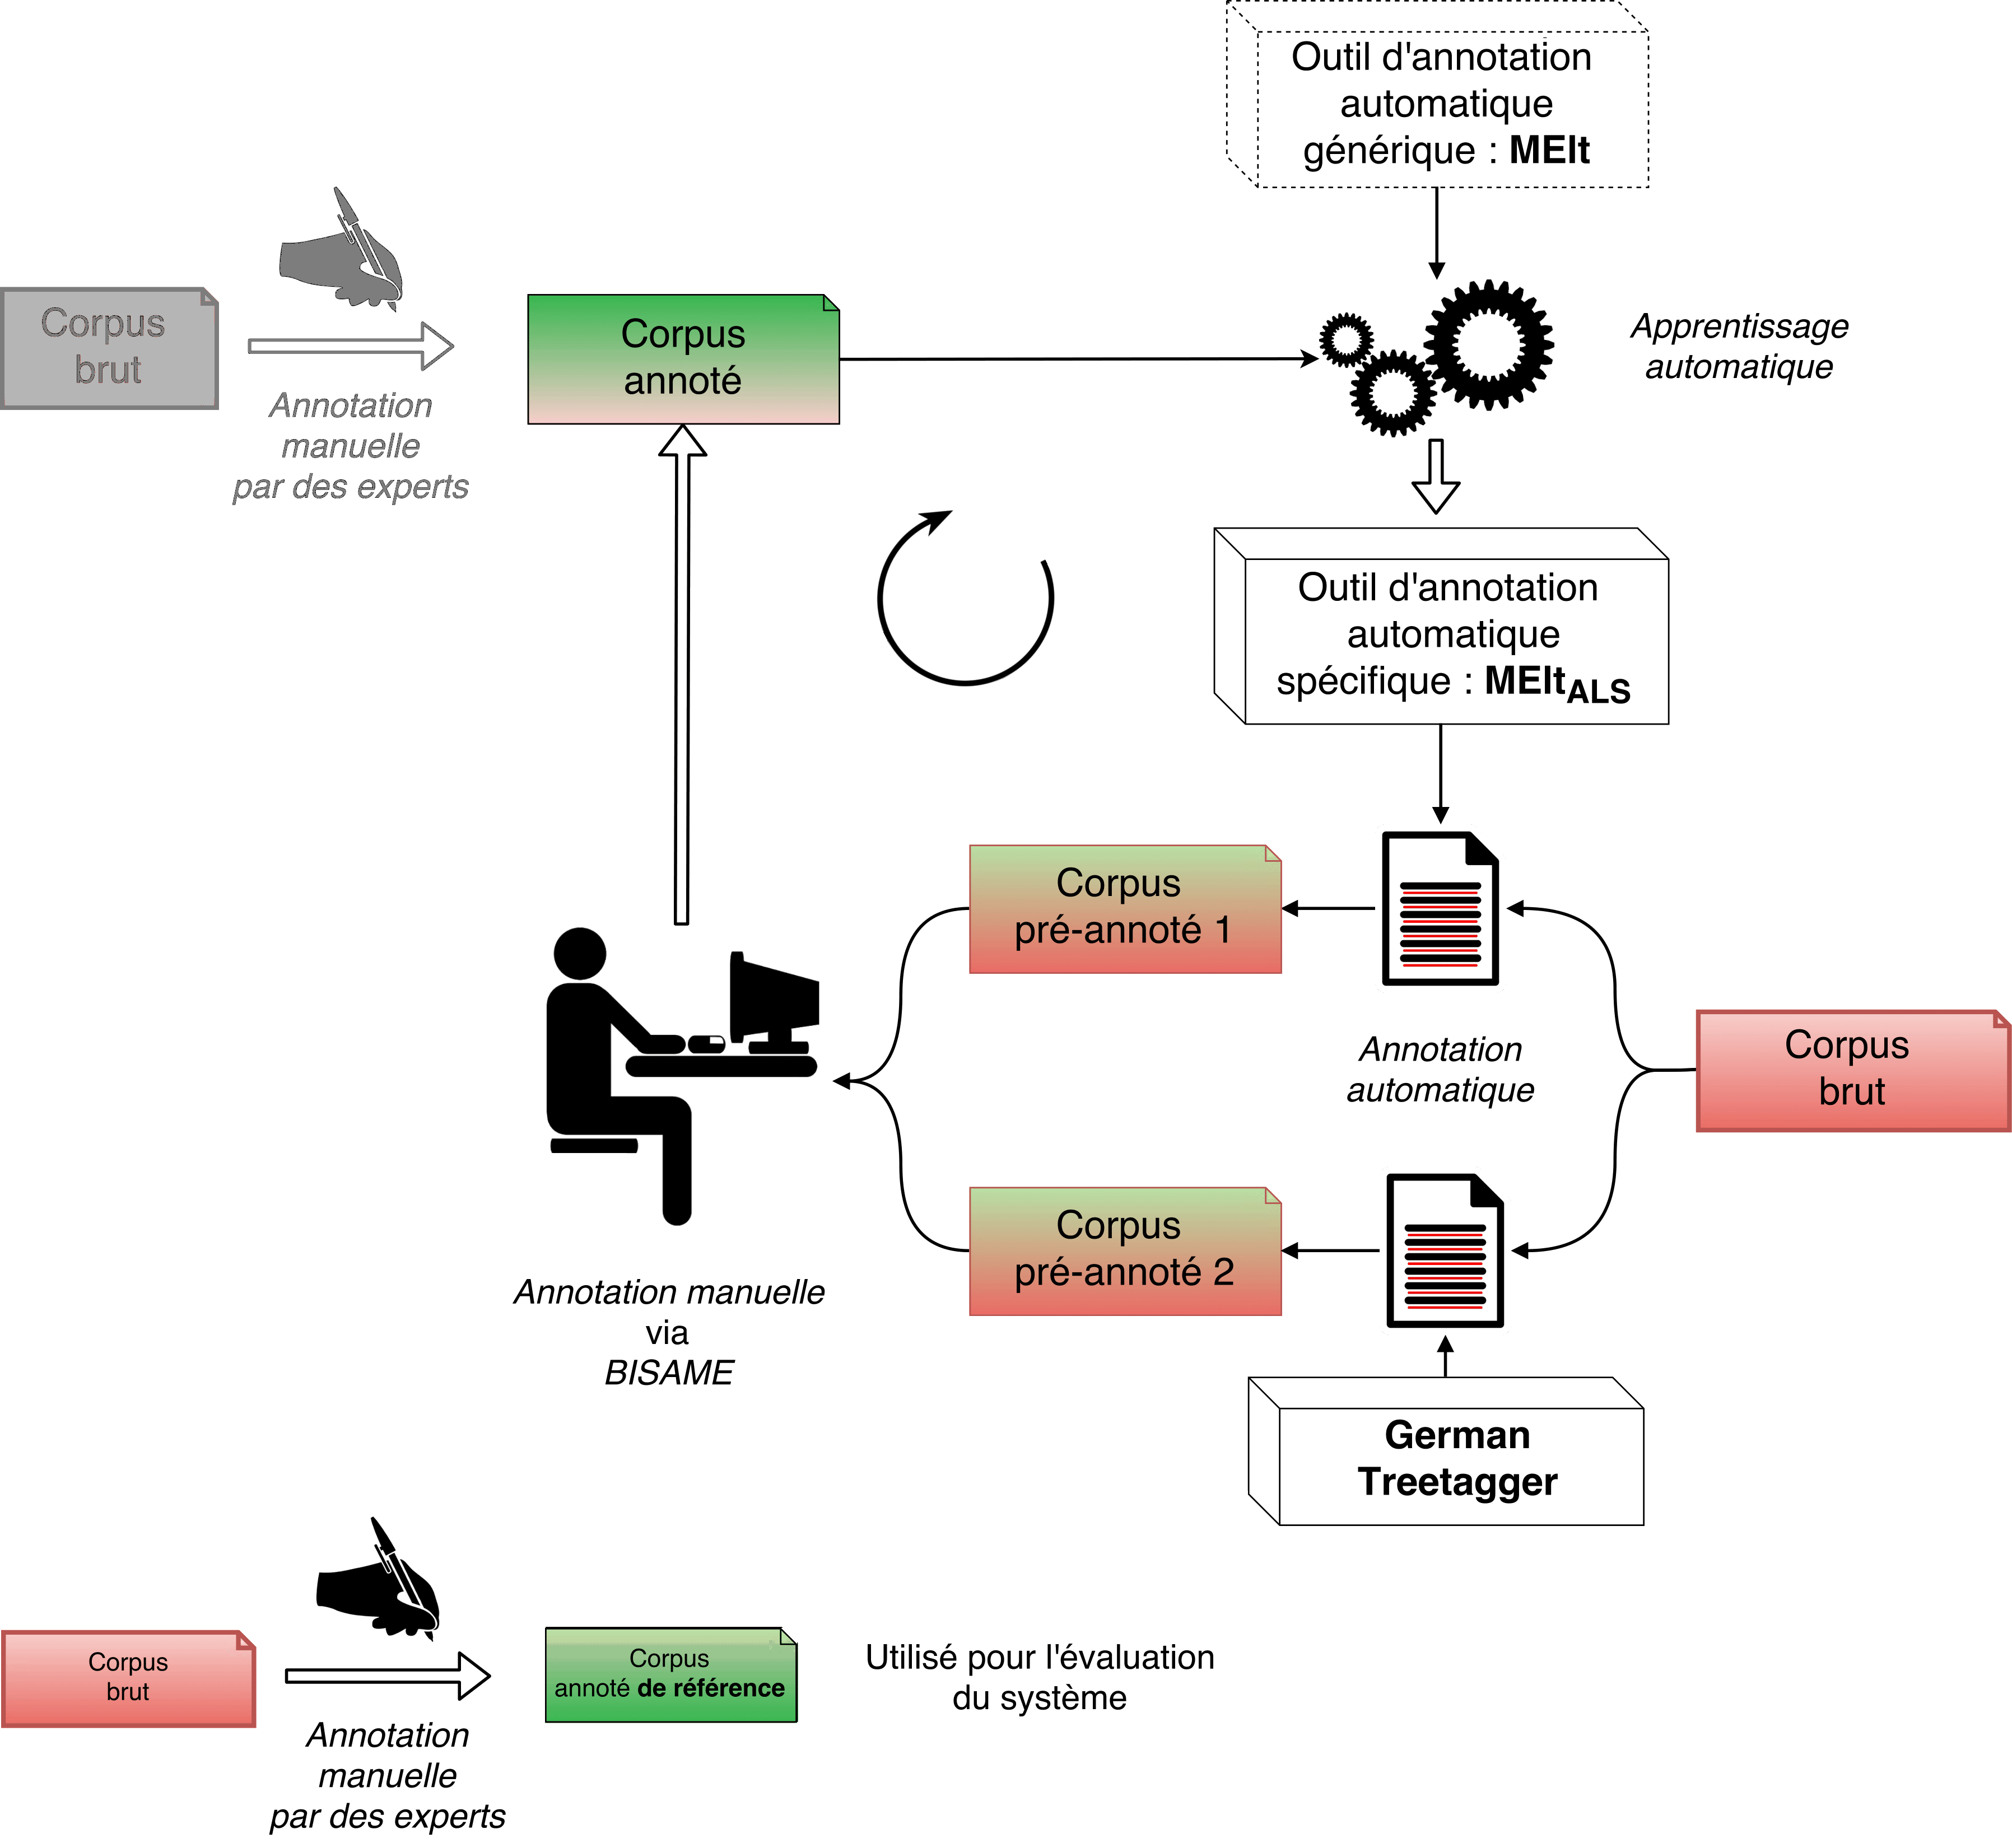
\includegraphics[width=0.8\linewidth]{figures/annotation-bisame-ref-2.png}
  \end{center}
    \hfill\cite{Fort2012} 
\end{frame}



\section{\tool{Bisame}\thinspace - une plate-forme d'annotation légèrement ludifiée}

\subsection{Présentation de la plate-forme}


\begin{frame}{\tool{Bisame}}
  \Wider[4em]{
    \begin{tikzpicture}
      \node (img0) {\includegraphics[width=1\textwidth]{figures/frontpage.png}};
      \pause
      \node (img1) at (img0) {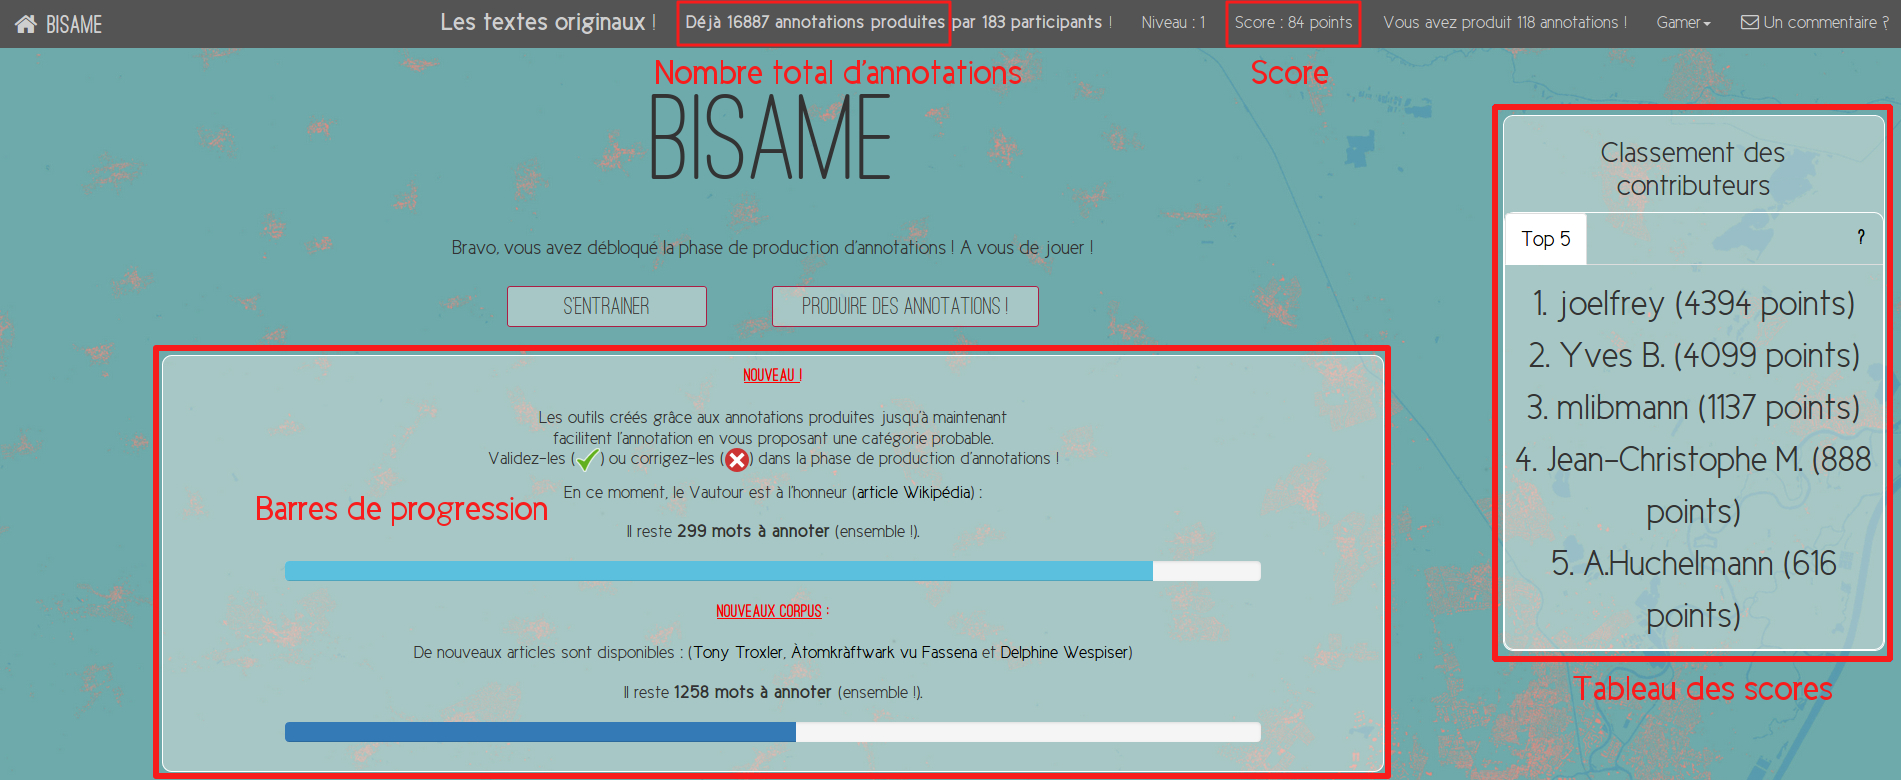
\includegraphics[width=1\textwidth]{figures/frontpage-fr.png}};
      \pause
      \node (img2) at (img0) {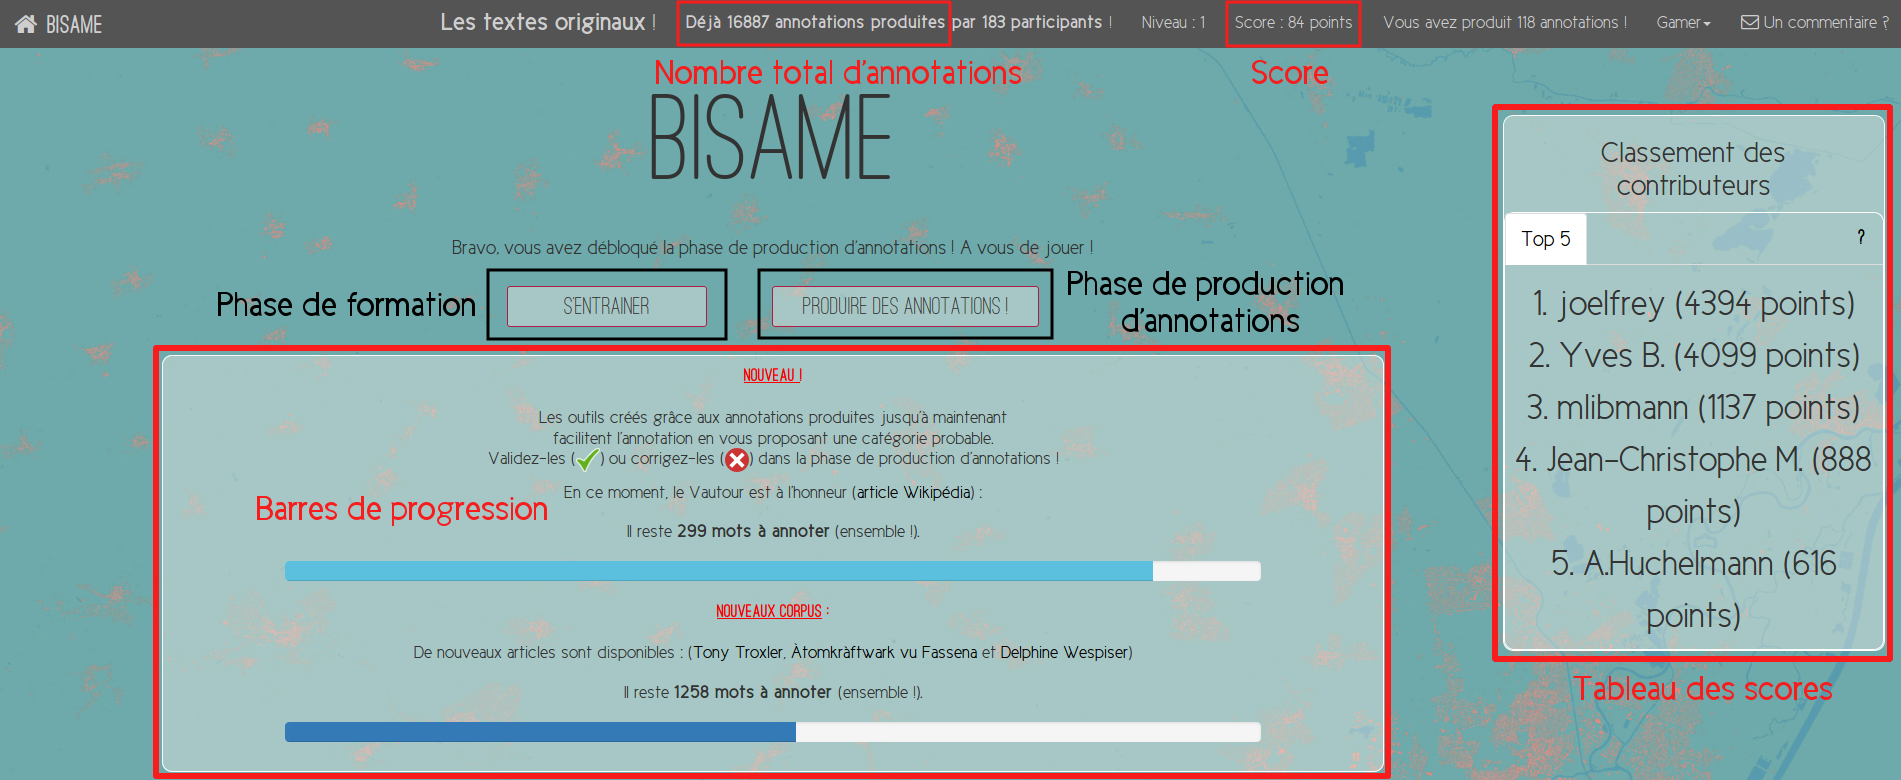
\includegraphics[width=1\textwidth]{figures/frontpage-fr-2.png}};
    \end{tikzpicture}  
  }   
\end{frame}

\begin{frame}{Annoter \textit{via} \tool{Bisame}}
  En fonction des résultats des deux outils de pré-annotation :
  \begin{center}
    Si \tool{Stanford Tagger} \textcolor{red}{!=} \tool{MElt$_{ALS}$}: \\
      \begin{figure}     
        \includegraphics[width=0.95\textwidth]{figures/annot2.png}
    \end{figure}
    \visible<2->{Si \tool{Stanford Tagger} \textcolor{greensolution}{\textbf{=}} \tool{MElt$_{ALS}$}: \\
      \begin{figure}   
        \includegraphics[width=0.95\textwidth]{figures/annot1.png}
      \end{figure}
    }    
  \end{center}
\end{frame}
\begin{frame}{Aide-mémoire \footnotemark[1]}
  \Wider[4em]{
  \begin{center}
      \begin{figure}     
        \includegraphics[width=0.3\textwidth]{figures/aide-memoire.png}
    \end{figure}
  \end{center}
  }
  \footnotetext[1]{Inspiré du guide d'annotation rédigé par~\cite{Bernhard2016}.}
\end{frame}

\begin{frame}{Phase de formation}
  \Wider[4em]{
  \begin{center}
      \begin{figure}     
        \includegraphics[width=1\textwidth]{figures/training.png}
    \end{figure}
  \end{center}
  }
\end{frame}

\begin{frame}{Phase de production d'annotations}
    \begin{itemize}
    \item 3 phrases issues du corpus brut
    \item 1 phrase issue du corpus de référence pour l'\textbf{évaluation régulière du participant}
    \end{itemize}
\end{frame}


%% synthèse des annotations obtenues
\subsection{Traitement des annotations obtenues}
\begin{frame}{Traitement des annotations concurrentes - 1}
  \centering
  \small  \textit{\textbf{Dr Mentelin hàt sina \uline{Stroßburger} Drukaréi grinda.}} (\og Mentelin a fondé son imprimerie strasbourgeoise \fg{}.)
  
  \begin{columns}
    \begin{column}{0.2\textwidth}
    \end{column}
    \begin{column}{0.2\textwidth}
      \textit{\textbf{{Stroßburger}}}
    \end{column}
    \begin{column}{0.2\textwidth}
      \visible<2->{
        \[
        \left\{
        \begin{tabular}{ccc}
          \textsc{propn} (participant P1) \\
          \textsc{adj} (participant P2, P3, P4)\\ 
          \textsc{noun} (participant P5) \\
        \end{tabular} 
        \right. \]}
    \end{column}
    \begin{column}{0.4\textwidth}
    \end{column}
  \end{columns}
  \centering
  \visible<3->{\small À chaque participant $P$ est associé score de confiance \\ (réévalué régulièrement) \\~\\   $Confiance_{P}=\frac{NbAnn_{Ref,Correcte}}{NbAnn_{Ref}}$} \\ \bigskip
  \visible<4->{\small $\rightarrow$ ce score de confiance est reporté sur les \textbf{annotations} effectuées : \\~\\  $ScoreAnn=Confiance_{P}$}
\end{frame}
    

\begin{frame}{Traitement des annotations concurrentes - 2}
  \centering
  \small calcul de l'étiquette la plus probable pour un token $T$: \\~\\
  \small $ScoreCat_{T,C_i}$=$1 - \prod_{j} (1-ScoreAnn_{T,U_j,C_i}))$ \\~\\
  \small et $C_{T}=\operatorname*{arg\,max}_i(ScoreAnn_{T,C_i})$                
  \begin{table}[!ht]
    \centering
    \resizebox{1\linewidth}{!}{
      \begin{tabular}{l|c|c}
        \toprule
        Catégorie choisie &  $ScoreAnn$  (Score de l'\textbf{annotation}) 
        & $ScoreCat$ (Score de la \textbf{catégorie})
        \\ \hline
        \textsc{propn}                & $0,935$      &          \visible<2->{$0,935$}       \\ \hline \hline
        \multirow{3}{*}{\textsc{adj}} & $0,875$       &         \visible<2->{\multirow{3}{*}{$\color{red} \mathbf{0,991}$}} \\ \cline{2-2}
        & $0,846$                                                \\\cline{2-2}
        & $0,938$                                                 \\ \hline \hline
        \textsc{noun}                 & $0,25$ & \visible<2->{$0,25$} \\ 
        \toprule
      \end{tabular}
    }
  \end{table}
  \centering
  \visible<2>{$\Rightarrow C_{\textbf{\textit{Stroßburger}}}=$\textsc{adj}}
\end{frame}


%%%% Résultats
\section{Résultats et analyse}
   
    %% \centering
    %%  \cite{Millour2017}

  %%     %\item \textbf{F-mesure} moyenne de \tool{Bisame} sur le \uline{corpus de référence} : \textbf{92~\%}.

  %% \visible<3->{
  %%   \begin{table}[h!]
  %%     \begin{tabular}{lcc}
  %%       \toprule
  %%       & \multicolumn{1}{l}{German \tool{TreeTagger}} & \multicolumn{1}{l}{\tool{MElt$_{ALS}$}} \\ \hline
  %%       \sla Pièce de théâtre     & 83~\%                                       & 66~\%                     \\ \hline
  %%       \nla Article Wikipédia & 85~\%                                       & 84~\%                   \\
  %%       \toprule
  %%     \end{tabular}
  %%   \end{table}
  %% }
  %% \footnotetext[1]{16~628 annotations ont été effectuées au total.}

%% Corpus annoté

\subsection{La participation}
\begin{frame}{La participation}
  \begin{figure}[h!tbp]
    \begin{center} 
      \begin{tikzpicture}
        \pgfplotsset{
	  width=0.88\textwidth,
	  height=0.33\textwidth,
	  axis x line=bottom,
        }
        \begin{axis}[
    	    axis y line*=left,
	    ybar=50pt,
	    bar width=0.1125cm,
	    ymin=0,	
	    ymax=45,
	    xlabel near ticks,
	    ylabel near ticks,
	    ystep=10,
	    %ymajorgrids,
	    %enlarge x limits=0.015,
	    minor tick num=0,
	    ylabel=Nb. participants actifs,
	    symbolic x coords={Mai,Ma2,Ma3,Ma4,Juin,Juin2,Juin3,Juin4,Juillet,Juil2,Juil3,Juil4,Août,Ao2,Ao3,Ao4,Septembre,Se2,Se3,Se4,Octobre,Oc2,Oc3,Oc4,Novembre,No2,No3,No4,Décembre,De2,De3,De4,Janvier,Ja2,Ja3,Ja4,Février,Fe2,Fe3,Fe4},
	    xtick=data,
            xticklabels={\empty,mai,\empty,\empty,\empty,juin,\empty,\empty,\empty,juillet,\empty,\empty,\empty,août,\empty,\empty,\empty,septembre,\empty,\empty,\empty,octobre,\empty,\empty,\empty,novembre,\empty,\empty,\empty,décembre,\empty,\empty,\empty,janvier,\empty,\empty,\empty,février},
            x tick label style={rotate=50, anchor=east},
    	    legend columns=-1,
	    scaled ticks=false,
          ]
          \addplot[black,fill=black!40,bar shift=-.055125cm,line width=0.05pt] table [
            y=Nb1
          ] {data/participants-and-annotations-per-week.dat};
          \label{participants};
        \end{axis}
        \begin{axis}[
	    ybar=0pt,
	    bar width=0.099cm,
	    ymin=0,	
	    ymax=4500,
            hide x axis,
            axis y line*=right,
	    xlabel near ticks,
	    ylabel near ticks,
	    ystep=1000,
	    ymajorgrids,
	    %enlarge x limits=0.05,
	    minor tick num=1,
	    ylabel=Nb. annotations,
	    symbolic x coords={Mai,Ma2,Ma3,Ma4,Juin,Juin2,Juin3,Juin4,Juillet,Juil2,Juil3,Juil4,Août,Ao2,Ao3,Ao4,Septembre,Se2,Se3,Se4,Octobre,Oc2,Oc3,Oc4,Novembre,No2,No3,No4,Décembre,De2,De3,De4,Janvier,Ja2,Ja3,Ja4,Février,Fe2,Fe3,Fe4},
	    xtick=data,
	    x tick label style={rotate=-55, anchor=west},
    	    legend columns=-1,
	    scaled ticks=false,
	    legend style={at={(1,1.4)}}
          ]
          \addlegendimage{/pgfplots/refstyle=participants,style={at={(2,3)}}}\addlegendentry{Nb. participants actifs} 
          \addplot[fill=black!70,bar shift=0.055125cm,line width=0.05pt]table [
            y=Nb2
          ] {data/participants-and-annotations-per-week.dat};
          \addlegendentry{Nb. annotations}
        \end{axis}
      \end{tikzpicture}
    \end{center}
  \end{figure}
  \vspace{-1.8cm}
  \hfill \includegraphics[width=0.5cm]{figures/caution.png} \\
  %%  \Wider[4em]{\begin{figure}[h!tbp]
  %%     \begin{center} 
  %%       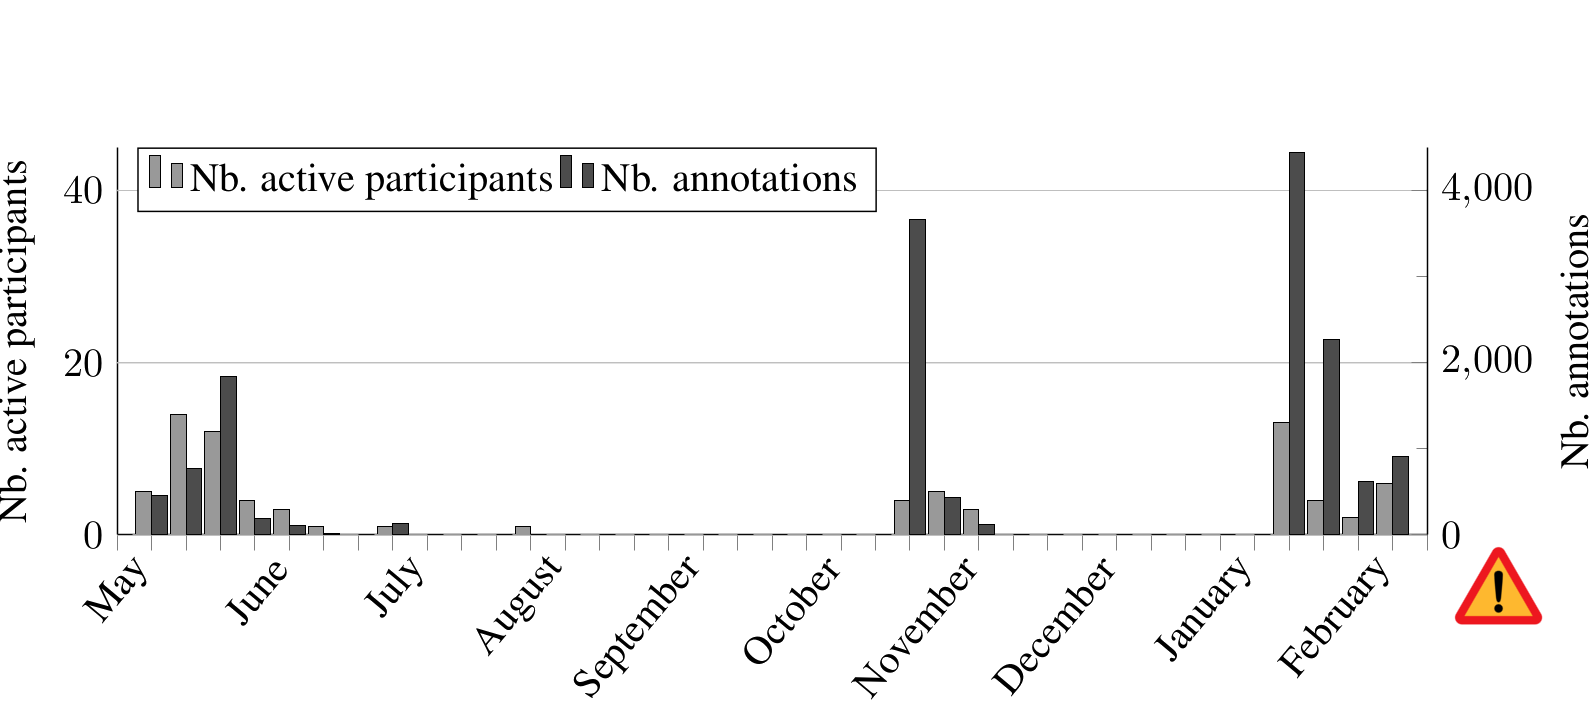
\includegraphics[width=1\textwidth]{figures/graphique-1-en.png}
  %%     \end{center}
  %% \end{figure}}
  %% \\
  %% \centering
  \bigskip
      \small mai 2016:  \small 29 participants ont produit 3~000 annotations \\
      \bigskip
      \visible<2->{\small janvier 2017 : 15 participants ont produit plus de 7~000 annotations}
\end{frame}

\subsection{Le corpus annoté}
\begin{frame}{Un nouveau corpus annoté de l'alsacien}
  %\Wider[3em]{
    \begin{itemize}
    \item \textbf{42 participants}
    \item \textbf{59} jours d'annotation
    \item \textbf{16~628 annotations}, dont :
      \begin{itemize}
        \item 8~833 sur le corpus brut (pour la production d'annotation)
        \item<2-> 7~795 sur le corpus de référence (pour l'évaluation)
      \end{itemize}
      \end{itemize}
  %}
    \visible<3->{$\rightarrow$ un nouveau corpus annoté de l'alsacien de \textbf{5~725 tokens}}\\
    %\visible<3->{$\rightarrow$ Un outil d'annotation en parties du discours entraîné avec 250 phrases : \textbf{\tool{MElt$_{\mathbf{ALS,250}}$}}.}
\end{frame}

%% MElt entraîné

\begin{frame}{Qualité du corpus annoté}
  \centering
  on calcule la \textbf{F-mesure} par catégorie sur le corpus de référence annoté, soit une mesure pondérée de la

  \textbf{précision} \\ \footnotesize (mesure du taux d'erreur de catégorisation pour une catégorie $C$ donnée) \\ \normalsize et du \textbf{rappel} \\ \footnotesize (proportion de tokens correctement identifiés pour une catégorie $C$ donnée)
\end{frame}

\begin{frame}{Qualité du corpus annoté}
 \bigskip
  \centering
  \Wider[2em]{\begin{figure}[h!tbp]
      \begin{center} 
        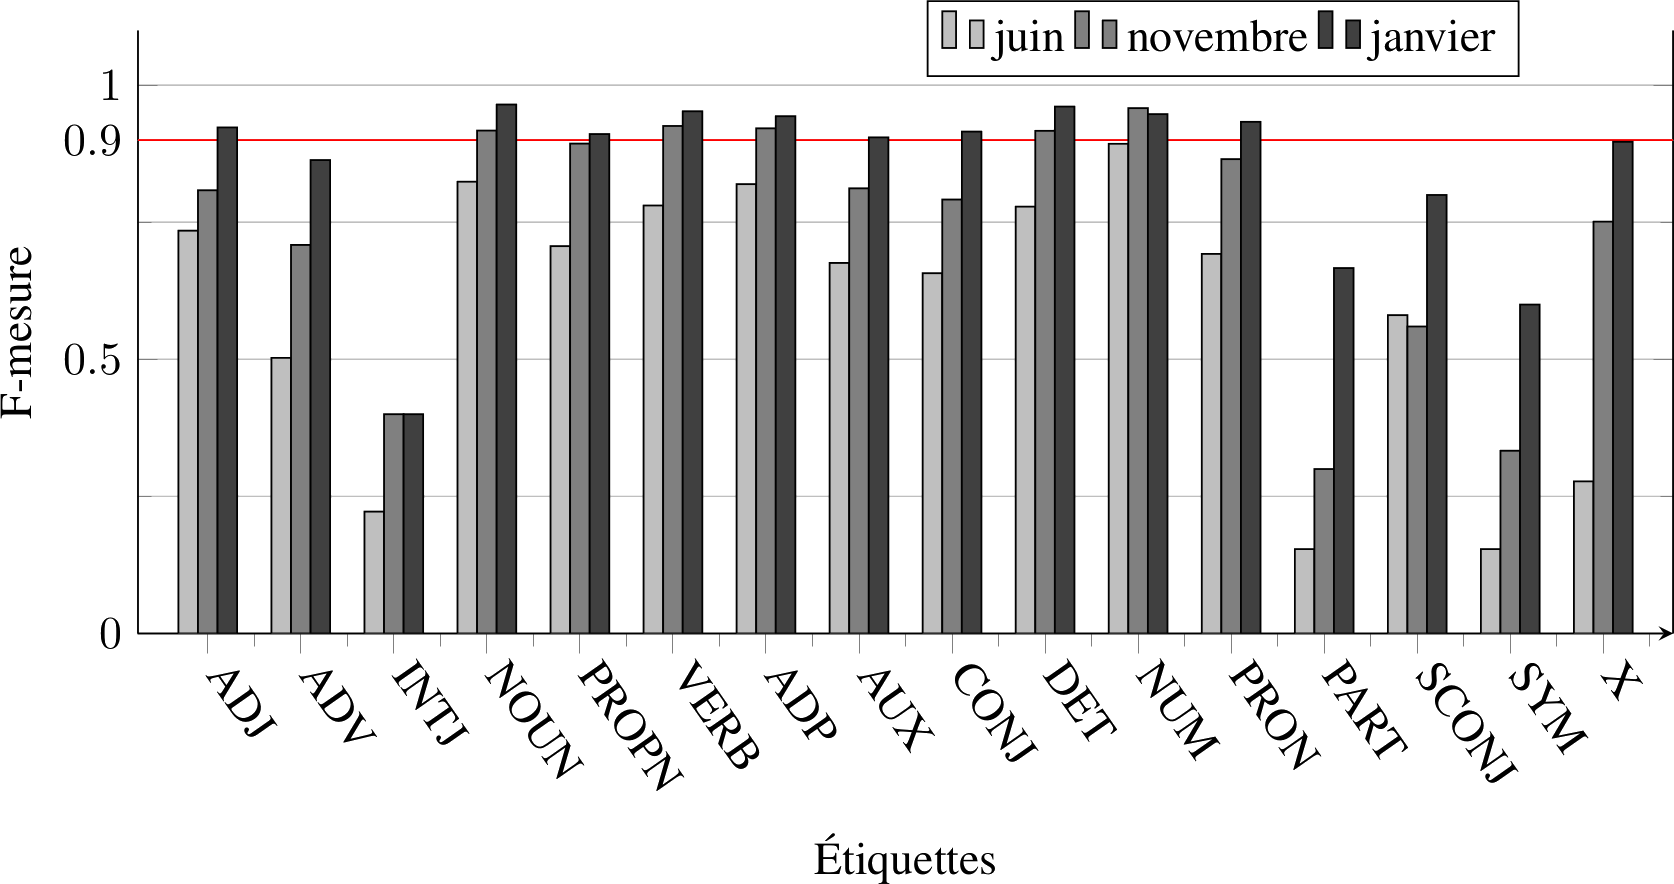
\includegraphics[width=1\textwidth]{figures/F-mesure.png}
      \end{center}
  \end{figure}}
  ~\\ \bigskip
    \centering 
  \textbf{F-mesure} moyenne de \tool{Bisame} : \textbf{93~\%} \\
\end{frame}

\subsection{L'outil d'annotation entraîné : \tool{MElt$_{ALS_{250}}$}}

\begin{frame}{Les performances de \tool{MElt$_{ALS}$}}
  \Wider[3em]{\begin{figure}[h!tbp]
      \begin{center} 
        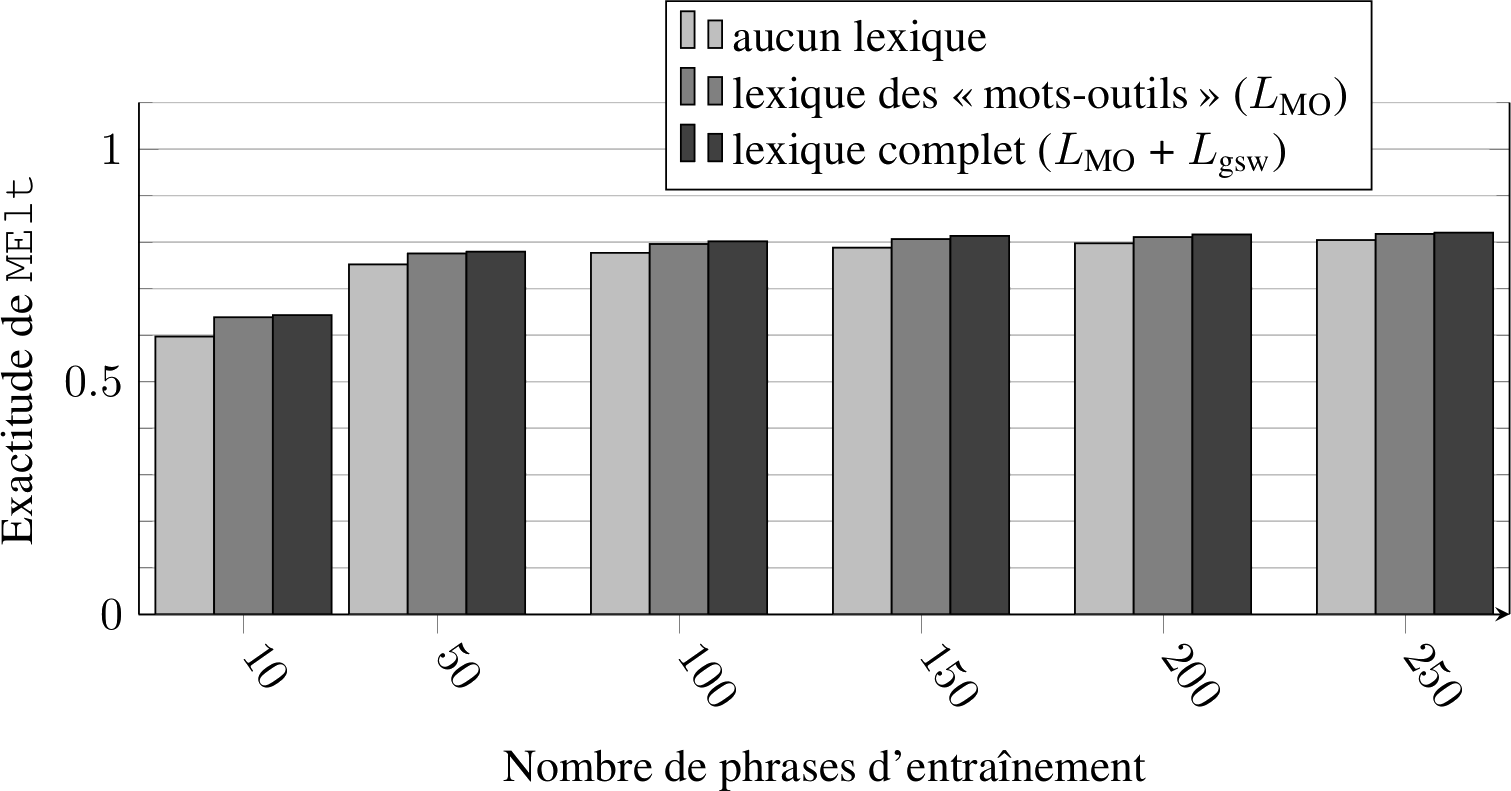
\includegraphics[width=0.8\textwidth]{figures/MElt.png}
      \end{center}
  \end{figure} 
    \centering
  \tool{MElt$_{ALS_{250}}$} atteint \textbf{82~\%} d'exactitude sur notre corpus de test\\
  
  }
\end{frame}

\begin{frame}{Les performances de \tool{MElt$_{ALS}$}}
      \centering

    \tool{MElt$_{ALS_{250}}$} atteint \textbf{82~\%} d'exactitude sur notre corpus de test\\~\\
    %\Wider[3em]{
    \small pour 10 phrases d'environ 10 mots, 2 mots par phrase sont mal annotés \\
  \scriptsize (\tool{MElt$_{FR}$} présente 97,7~\% d'exactitude \cite{Denis2010})  \\~\\

  \visible<2>{\normalsize les performances du \tool{Stanford Tagger}  sur l'alsacien sont presque atteintes mais c'est encore très insuffisant}

\end{frame}


\begin{frame}{Les performances de \tool{MElt$_{ALS}$}}
  \centering
  les meilleures performances sont obtenues sur les textes appartenant à la même variante que le corpus d'entraînement (haut alémanique du sud)
   \begin{table}[h!]
      \begin{tabular}{lcc}
        \toprule
        & \multicolumn{1}{l}{\tool{Stanford tagger}} & \multicolumn{1}{l}{\tool{MElt$_{ALS_{250}}$}} \\ \hline
        \sla Pièce de théâtre     & 83~\%                                       & \textbf{66~\%}                     \\ \hline
        \nla Article \tool{Wikipédia} & 85~\%                                       & \textbf{84~\%}                   \\
        \toprule
      \end{tabular}
    \end{table}
\end{frame}

\begin{frame}{Conclusion et perspectives}
  \centering
  la méthodologie développée est prometteuse mais perfectible
  \Wider[2em]{    
  \vspace{0.8cm}
  \begin{itemize}
  \item<2->  \small manque de variété des corpus disponibles \visible<3->{\textbf{\normalsize \color{greensolution} $\rightarrow$  permettre la soumission de \textbf{textes personnels}~\cite{Liberm2016} }}
   \visible<4->{\item  \small qualité d'annotation encore imparfaite} \visible<5->{\textbf{ \normalsize \color{greensolution}$\rightarrow$  repenser le guide d'annotation et la phase de formation} }
  \end{itemize}
  }
\end{frame}

\begin{frame}{Conclusion et perspectives}
  \centering
  La méthodologie est prometteuse mais perfectible
  \Wider[2em]{    
    \vspace{0.8cm}
    \begin{itemize}
    \item  \small aspect ludique insuffisant pour maintenir \textbf{motivation} \visible<2->{et \textbf{volition}} \visible<3->{\textbf{\normalsize \color{greensolution} { \visible<3->{$\rightarrow$~développer de nouvelles fonctionalités ludiques \og classiques \fg{}} \\
           \visible<4->{$\rightarrow$ jouer sur le sentiment d'appartenance à la communauté dialectophone} \\
           \visible<5->{$\rightarrow$ améliorer l'autonomie de la plate-forme (e-mails de rappel, \og une phrase par jour \fg{})}}}}
    \end{itemize}
  }
  \begin{center}
    \visible<1>{\og capacité à \textbf{attirer} des participants \fg{}}\\
    \visible<2>{\og capacité à \textbf{faire revenir} des participants~\cite{Fenouillet2009} \fg{}}
  \end{center}
\end{frame}

\begin{frame}{Conclusion et perspectives}
  \centering
  La méthodologie est prometteuse mais perfectible
  \Wider[2em]{    
  \vspace{0.8cm}
    \begin{itemize}
      %\item Reinforce community feeling \textit{within} the platform thanks to \textbf{social incentives}. %as they have been appreciated so far and have proved their efficiency elsewhere
    \item adapter le jeu d'étiquettes universel aux spécificités de l'alsacien
    \item<2-> travailler à une meilleure intégration de la diversité dialectale et orthographique
    \item<3-> adapter la plate-forme à une autre langue peu dotée : le créole guadeloupéen (\small projet en cours avec Gwladys Feler, étudiante en Master 1)
      %\item<2-> Try to manage better dialectal diversity in the written form. % and I take advantage of this talk to say that if you have some references on the subject I would me really glad to have them ! 
    \end{itemize}
  }
\end{frame}

\begin{frame}[standout]
  \textit{Merci vielmols!} \\~\\
  \begin{center}
    %{\setstretch{1.5}
    \normalsize
    \tool{Bisame}: \url{http://bisame.herokuapp.com} \\ 
    
    \includegraphics[width=0.02\textwidth]{figures/github-white.png}\enspace Github:         \url{https://github.com/alicemillour/Bisame}
    %}
  \end{center}
\end{frame}

%\appendix

%\begin{frame}[fragile]{Backup slides}
%  Sometimes, it is useful to add slides at the end of your presentation to
%  refer to during audience questions.
%
%  The best way to do this is to include the \verb|appendixnumberbeamer|
%  package in your preamble and call \verb|\appendix| before your backup slides.
%
%  \themename will automatically turn off slide numbering and progress bars for
%  slides in the appendix.
%\end{frame}

\begin{frame}[allowframebreaks]{References}

  \bibliographystyle{apalike}
  \bibliography{pres_atelier_corpus}
\end{frame}


\end{document}
